\chapter{几何背景中的自由场与量子态}\label{chap:ghs-geometric-free-states}
\label{chap:ghs-quantum-boundary-states}
\label{chap:ghs-free-field-arbitrary-slice}
\label{chap:ghs-state-operator-general-setting}
\label{chap:ghs-causal-field-algebra}
\label{chap:ghs-r6-hyperbolic-symplectic}
\label{chap:ghs-lorentzian-general}

平直空间的量子场论已经给出了传播子、Fock 空间和散射振幅。带边界或曲率的空间首先改变的却不是相互作用顶角，而是自由场的空间算子：同一个微分表达式在不同定义域上可以有不同的零模、负模与谱。只有先固定这个算子，才知道哪些模能够作为正频振子，以及高斯真空是否存在。

前章的一般截面量子化使这个问题可以从谱演算出发。欧氏传播核给出边界场之间的高斯传递；反射正性把其中的半正定配对变成量子态内积。真实时间的发展还要求因果传播和守恒辛形式。它们确定场代数，兼容复结构才进一步选择正频、真空和粒子。这样得到的量子态随后必须满足短距离正则性，才允许定义局域复合算符。

\begin{definition}[几何量、物理时间与场归一化]
黎曼截面的度规 $h$ 正定，$\Delta_h=\operatorname{div}_h\nabla_h$ 为非正算子；复内积采用物理约定 $\langle f,g\rangle=\int\overline f g\dd\mu_h$，对第二变量线性。空间谱算子 $A$ 的本征值具有 $L^{-2}$ 量纲。长度坐标 $x^0=ct$、长度型欧氏时间 $u_E$ 和热核参数 $s$ 分别具有 $L,L,L^2$ 量纲，$\exp(-sA)$ 与 $\exp(-u_E\sqrt A)$ 是不同半群。无量纲作用量记为 $\mathscr I=I_E/\hbar$，场的规范化长度维数为 $L^{(2-d)/2}$。

洛伦兹度规固定为 $(+,-,\ldots,-)$，曲率约定为 $[\nabla_c,\nabla_d]v^a=R^a{}_{bcd}v^b$，$\mathcal R_L=g_L^{bd}R^a{}_{bad}$。在超静态积上 $\mathcal R_L=-\mathcal R_h$。因此与欧氏势 $\mu^2+\xi\mathcal R_h$ 相容的 Lorentz 方程写成 $P=\Box_{g_L}+\mu^2-\xi\mathcal R_L$。$\mu=mc/\hbar$，曲率耦合 $\xi$ 无量纲。若截面以参考半径 $R$ 缩放，$A_{\rm phys}=R^{-2}A$，物理频率为 $c\sqrt\lambda/R$，激发能量为 $\hbar c\sqrt\lambda/R$。
\end{definition}

\section{传播核与边界态}
\label{sec:ghs-euclidean-boundary-kernels}


\begin{definition}[振子坐标与核测度的单位换算]
本节的 $\tau,T$ 为长度型欧氏时间，$\omega$ 为逆长度谱频率，$q$ 是满足 $[q,p]=\ii$ 的规范化坐标，$[q]=L^{1/2}$、$[p]=L^{-1/2}$。因此 $\omega T$ 与 $\omega q^2$ 无量纲，指数中的经典作用量是 $\mathscr I_{\rm cl}=I_{E,\rm cl}/\hbar$。坐标核按 $\dd q$ 归一。

对质量 $M$ 的物理位移 $Q$，令 $q_{\rm phys}=\sqrt M Q$、$p_{\rm phys}=P_Q/\sqrt M$，则
\[
 q_{\rm phys}=\sqrt{\hbar/c}\,q,\qquad p_{\rm phys}=\sqrt{\hbar c}\,p,\qquad T_{\rm phys}=T/c,\qquad
 \omega_{\rm phys}=c\omega,\qquad K_{\rm phys}=\sqrt{c/\hbar}\,K.
\]
这些变换使 $[q_{\rm phys},p_{\rm phys}]=\ii\hbar$，并保持 $K\dd q=K_{\rm phys}\dd q_{\rm phys}$。后面的有限模 Schur 积分与含 $\hbar$ 的振子例题使用物理质量加权坐标；随后返回 $\mathscr I=I_E/\hbar$ 的场论规范化。
\end{definition}

现在将欧氏时间限制在 $0\le\tau\le T$，并且在两端固定场的配置 $f_0,f_T$。路径积分
\[
 K_T[f_T,f_0]=\int_{\varphi(0)=f_0}^{\varphi(T)=f_T}
 \mathcal D\varphi\;\ee^{-\mathscr I_E[\varphi]}
\]
首先应作为有限模截断下的高斯积分理解。它不是 $G$：$G$ 是两个场插入点的协方差，而 $K_T$ 是从一个完整边界场配置传播到另一个配置的振幅核。两者由同一二次算子决定，但边界数据的角色不同。

\begin{example}[精确 Mehler 边界核]
对一个频率为 $\omega>0$ 的模，经典方程为 $\ddot q=\omega^2q$，边界条件 $q(0)=q_0$、$q(T)=q_T$。写出满足两个端点条件的唯一经典解：
\begin{equation}\label{eq:ghs-bridge-classical-path}
 q_{\rm cl}(\tau)=
 \frac{\sinh[\omega(T-\tau)]}{\sinh(\omega T)}q_0
 +\frac{\sinh(\omega\tau)}{\sinh(\omega T)}q_T.
\end{equation}
在经典路径上，$\dot q^2+\omega^2q^2=\partial_\tau(q\dot q)$。故作用量不必再积分两个平方，而可化为端点项
\[
 \mathscr I_{\rm cl}=\frac12[q\dot q]_0^T
 =\frac{\omega}{2\sinh(\omega T)}
 \left[(q_0^2+q_T^2)\cosh(\omega T)-2q_0q_T\right].
\]
二次涨落的行列式给出标准 Mehler 核，因此
\begin{equation}\label{eq:ghs-bridge-Mehler}
 K_T(q_T,q_0)=
 \sqrt{\frac{\omega}{2\pi\sinh(\omega T)}}
 \exp\left[-\frac{\omega}{2\sinh(\omega T)}
 \bigl((q_0^2+q_T^2)\cosh(\omega T)-2q_0q_T\bigr)\right].
\end{equation}
\end{example}

这里的哈密顿量 包括 $\omega/2$ 的零点能。把两个区间拼起来，便有
\begin{equation}\label{eq:ghs-bridge-kernel-gluing}
 \int_{\RR}K_{T_2}(q_2,q)K_{T_1}(q,q_0)\,\dd q
 =K_{T_1+T_2}(q_2,q_0).
\end{equation}
这条拼接律正是熟悉的 $\ee^{-T_2H}\ee^{-T_1H}=\ee^{-(T_1+T_2)H}$ 在坐标核中的表现。



\begin{proof}
记 $a=\omega T_1$、$b=\omega T_2$。把两个核指数相加，关于中间坐标 $q$ 的部分为 $-\frac12 A_q q^2+B_qq$，其中
\begin{align*}
 A_q&=\omega(\coth a+\coth b)
 =\omega\frac{\sinh(a+b)}{\sinh a\sinh b},\\
 B_q&=\omega\left(\frac{q_0}{\sinh a}+\frac{q_2}{\sinh b}\right).
\end{align*}
高斯积分 $\int\ee^{-A_qq^2/2+B_qq}\dd q=\sqrt{2\pi/A_q}\,\ee^{B_q^2/(2A_q)}$。用
$\sinh(a+b)=\sinh a\cosh b+\cosh a\sinh b$ 合并平方项，可得合成指数
\[
 -\frac{\omega}{2\sinh(a+b)}
 [(q_0^2+q_2^2)\cosh(a+b)-2q_0q_2].
\]
归一化前因子也合并为 $\sqrt{\omega/[2\pi\sinh(a+b)]}$，于是恢复 \cref{eq:ghs-bridge-Mehler}，其中 $T=T_1+T_2$。
\end{proof}

式 \cref{eq:ghs-bridge-Mehler} 中的非对角项 $-2q_0q_T$ 在 $T\to\infty$ 时指数衰减：两端的数据逐渐失去耦合。对一般截面，把 $\omega$ 替换成每个 $\sqrt{A}$ 的谱频率，就得到无限个边界振子的传递核；其涨落行列式在无限维下需另行正则化。把 $T$ 换成球面半径的对数只是特殊共形几何中的进一步步骤，尚不能称为一般流形上的径向量子化。

\begin{figure}[htbp]
\centering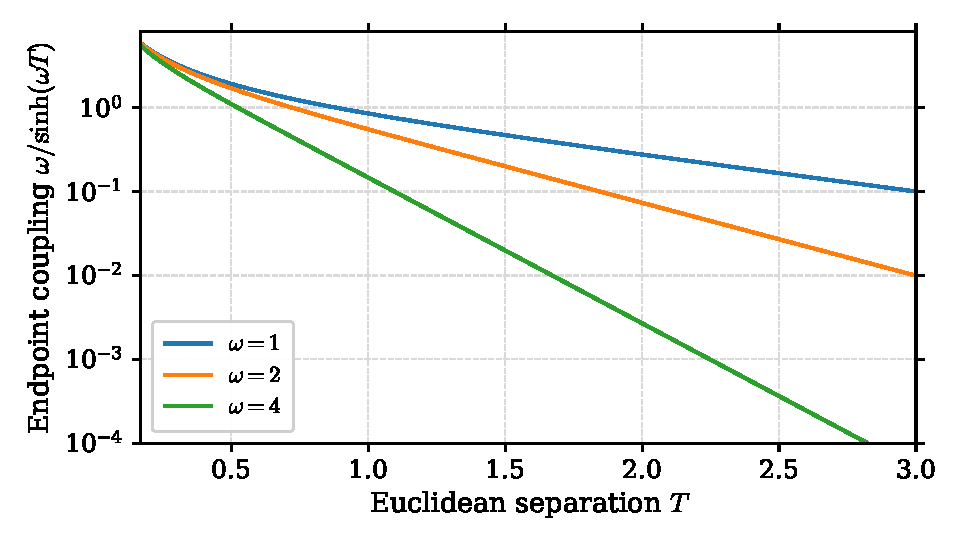
\includegraphics[width=.82\linewidth]{content/FreeElectronQuantumOptics/figures/geometry-highspin/generated/boundary_mode_gluing.pdf}
\caption{正自伴空间算子的单模边界传递系数 $\omega/\sinh(\omega T)$。高频模更快地丧失两端边界数据的耦合；该衰减来自 \cref{eq:ghs-bridge-Mehler} 的精确二次型，图中各曲线仅取不同 $\omega$，未作额外近似。}\label{fig:ghs-bridge-boundary-gluing}
\end{figure}


前面的传播核是算子表达式。为了看清楚它如何用于一次完整计算，令空间截面是一条周长为 $L$ 的平直圆周，坐标 $x\in[0,L)$、周期条件 $f(x+L)=f(x)$。这条圆周既是最简单的紧致空间，也说明了“空间有周期边界”和“空间真的有边界”是不同的几何：$x=0$ 与 $x=L$ 表示同一个点，并不提供两份独立的边界数据。

空间算子取 $A=-\partial_x^2+\mu^2$。本征问题 $Au=\lambda u$ 的一般复指数解 $\ee^{\ii kx}$ 满足周期条件恰在 $kL=2\pi n$ 时成立，$n\in\ZZ$。令
\begin{equation}\label{eq:ghs-bridge-circle-modes}
 u_n(x)=\frac1{\sqrt L}\ee^{2\pi\ii nx/L},\qquad
 \omega_n=\sqrt{\left(\frac{2\pi n}{L}\right)^2+\mu^2},
\end{equation}
则 $\int_0^L\overline{u_n}u_m\dd x=\delta_{nm}$，而
$\sum_nu_n(x)\overline{u_n(y)}=\delta_L(x-y)$，其中 $\delta_L$ 是周期的 delta 分布。由于这些本征函数是复数，实场的经典模系数满足 $q_{-n}=\overline{q_n}$；若改用实数的正弦、余弦基，每个 $n>0$ 恰给两个独立的实振子。它们在谱计数时应算两重，而不能把 $n$ 与 $-n$ 误当成两个无关的复标量粒子。

把 \cref{eq:ghs-bridge-circle-modes} 代入一般传播核，得到完全确定的二点函数
\begin{equation}\label{eq:ghs-bridge-circle-G}
 G(\tau,x;\tau',y)=\frac1L\sum_{n\in\ZZ}
 \frac{\ee^{-\omega_n|\tau-\tau'|}}{2\omega_n}
 \ee^{2\pi\ii n(x-y)/L}.
\end{equation}
配对 $n$ 与 $-n$ 以后，右侧显然是实函数。若 $|\tau-\tau'|>0$，高频模指数衰减，故该级数绝对收敛；在等时和同点极限则可能出现紫外奇性，不能直接把它当成处处有界的普通函数。

将两个场取在同一个空间点 $x=y$，只保留 $n=0$ 模便得到下界
\[
 G(\tau,x;\tau',x)\ \geq\frac{\ee^{-\mu|\tau-\tau'|}}{2L\mu}
 \qquad(\mu>0).
\]
这里所有求和项都是正的。若先取 $\tau\ne\tau'$ 再令 $\mu\to0^+$，该下界就发散。这不是短距离紫外发散：它完全由空间上不随 $x$ 改变的\emph{零模}引起。对于严格无质量的圆周标量，零模不受回复势限制，成为自由粒子而不是谐振子，因而不存在通常意义下的归一化高斯基态。这是为何一般空间量子化经常必须在构造 Fock 真空前先分离零模。

若将圆周半径不断增大，即 $L\to\infty$，固定物理距离 $x-y$ 与时间差，波数间距 $\Delta k=2\pi/L$ 变小。利用 Riemann 和极限，得到
\[
 \frac1L\sum_{n\in\ZZ}F(2\pi n/L)
 =\frac1{2\pi}\sum_n\Delta k\,F(k_n)
 \longrightarrow\int_\RR\frac{\dd k}{2\pi}F(k).
\]
因此 \cref{eq:ghs-bridge-circle-G} 回到熟悉的无限直线动量积分。这一计算明确展示了\emph{离散谱和连续谱只是空间性质不同造成的两种谱测度}，并不是两套无关的量子化规则。


我们已经会从空间本征值构造欧氏二点函数，但还没有说明为什么对欧氏时间进行这种计算，最后能够得到具有正范数的量子态。普通欧氏协方差的核正定性仍不够；为了由负时间区域反射到正时间区域，需要检验一条更强的性质。对自由场，它可以直接由 \cref{eq:ghs-bridge-spectral-G} 的每个正频模算出。

定义欧氏时间反射 $\theta(\tau,y)=(-\tau,y)$。取任意有限组位于正半时间 $\tau_i>0$ 的实试验函数 $f_i(y)$ 及复数 $c_i$，构造反射二次型
\[
 Q=\sum_{i,j}\overline{c_i}c_j
 \int_{\Sigma\times\Sigma}\overline{f_i(y)}
 G(-\tau_i,y;\tau_j,y')f_j(y')\dd\mu_h(y)\dd\mu_h(y').
\]
由于 $\tau_i,\tau_j>0$，反射点与原点的时间差是 $\tau_i+\tau_j$，不能写成 $|\tau_i-\tau_j|$。将谱表达代入并定义 $f_{ij}=\langle u_j,f_i\rangle$，得到
\begin{align*}
 Q&=\sum_{i,k}\overline{c_i}c_k\sum_j
 \frac{\ee^{-\omega_j(\tau_i+\tau_k)}}{2\omega_j}
 \overline{f_{ij}}f_{kj}\\
 &=\sum_j\frac1{2\omega_j}
 \left|\sum_i c_i\ee^{-\omega_j\tau_i}f_{ij}\right|^2\ge0.
\end{align*}
这样我们没有借助抽象的重建定理，就已经看到每个正频模怎样贡献一个非负平方。相应的反射正性就是从欧氏路径积分构造物理 Hilbert 空间所需的核心条件之一。

上述证明依赖 $A>0$，并使用了平移不变的欧氏时间以及二次高斯作用量。对于一般依赖时间的几何、含有复杂相互作用的场，或者没有适当反射对称性的空间，这种逐模平方不一定存在。反射正性必须作为独立的物理条件进行检验，不能因为写出了形式上的 $\ee^{-\mathscr I}$ 就自动宣称存在单位量子理论。


如果 $\Sigma=S^{n}$，角向微分算子的本征函数恰好是球谐，且简并度受旋转群保护。若 $\Sigma$ 是二维环面，模态是满足周期条件的 Fourier 波；若是缺少连续对称性的弯曲紧空间，谱通常依然离散，却没有一个自然的角动量标号。高自旋张量场的情况更进一步：场不仅是一个函数，而且每个点上的分量要在坐标变换下按张量规律混合，因而其微分算子必须带有联络与曲率信息。

这些模态计算所需的导数、积分与自伴定义域已由前章固定；更细的曲率交换和球谐表示可参照《数学技巧》与《群论》的对应章节。现在的问题是把精确边界核的归一化、量子态正性和真实时间传播放进同一场论中，因而必须继续计算行列式并明确因果初值。

\subsection{有限模边界核的行列式归一化}
\label{subsec:ghs-r6-gaussian-gluing}

有限模核计算在有限维普通积分与一维振子上推导边界拼接。一般场的泛函积分并不存在与有限维 Lebesgue 测度完全相同的平移不变测度，因此下面的有限模截断是严格代数计算；取无限模极限前必须再检查 Fredholm 行列式、零模与重整化。

\begin{example}[Schur 消元与行列式归一化]

设 $x\in\RR^n$ 是保留的边界变量，$y\in\RR^m$ 是待积分的内部变量，二次型写为
\[
Q(x,y)=\frac12x^{\mathsf T}Ax+x^{\mathsf T}By+
\frac12y^{\mathsf T}Cy,
\]
其中 $A=A^{\mathsf T}$，$C=C^{\mathsf T}>0$，且 $B$ 是 $n\times m$ 矩阵。引入 $z=y+C^{-1}B^{\mathsf T}x$，逐项展开
\begin{align*}
\frac12z^{\mathsf T}Cz
&=\frac12y^{\mathsf T}Cy+y^{\mathsf T}B^{\mathsf T}x
+\frac12x^{\mathsf T}BC^{-1}B^{\mathsf T}x,\\
Q(x,y)&=\frac12x^{\mathsf T}(A-BC^{-1}B^{\mathsf T})x
+\frac12z^{\mathsf T}Cz.
\end{align*}
对 $z$ 做正交对角化 $C=O^{\mathsf T}\operatorname{diag}(\lambda_1,\ldots,\lambda_m)O$，积分测度的 Jacobian 因 $O$ 正交而为 $1$，于是
\begin{equation}\label{eq:ghs-r6-schur-integral}
\int_{\RR^m}\exp\!\left(-\frac{Q(x,y)}\hbar\right)\dd^my
=\frac{(2\pi\hbar)^{m/2}}{\sqrt{\det C}}
\exp\!\left[-\frac1{2\hbar}x^{\mathsf T}(A-BC^{-1}B^{\mathsf T})x\right].
\end{equation}
因此积分消元同时改变两个数学对象：指数中的有效二次型和积分前的行列式归一化。只计算 Schur 补而不保存行列式，将丢失真空能及边界核拼接时的必要系数。

\end{example}

\begin{example}[物理单位中的 Mehler 核]

取质量加权的正则坐标 $q=\sqrt M Q$，$p=P_Q/\sqrt M$；这保持 $[q,p]=\ii\hbar$，$[q^2]=\mathrm{kg}\,\mathrm m^2$，$\omega$ 为每秒计的角频率，$T$ 为欧氏物理时间。给定实端点 $q(0)=q_i$、$q(T)=q_f$，欧氏振子作用量为
\[
I[q]=\frac12\int_0^T(\dot q^2+\omega^2q^2)\dd\tau,
\quad \omega>0.
\]
变分给出 $\ddot q=\omega^2q$。用端点数据解出
\[
q_{\mathrm{cl}}(\tau)=\frac{\sinh[\omega(T-\tau)]}{\sinh(\omega T)}q_i
+\frac{\sinh(\omega\tau)}{\sinh(\omega T)}q_f.
\]
在经典解上 $\dd(qq')/\dd\tau=q'^2+\omega^2q^2$，所以整个积分化为端点项：
\begin{align*}
I[q_{\mathrm{cl}}]
&=\frac12[q_{\mathrm{cl}}\dot q_{\mathrm{cl}}]_0^T\\
&=\frac\omega{2\sinh(\omega T)}
\left[(q_i^2+q_f^2)\cosh(\omega T)-2q_iq_f\right].
\end{align*}
其中交叉项的负号说明在两端固定同号位移时，最小经典作用量较小；这一特征正是边界传递算子的非对角负项。

端点指数只决定核的 $q$ 依赖，前置常数还须由热方程确定。对量子哈密顿量
$\widehat H=-(\hbar^2/2)\partial_q^2+(\omega^2/2)q^2$，欧氏核定义为 $K_T(q_f,q_i)=\langle q_f|\ee^{-T\widehat H/\hbar}|q_i\rangle$，满足
\[
\partial_TK_T=\frac\hbar2\partial_{q_f}^2K_T
-\frac{\omega^2q_f^2}{2\hbar}K_T,
\qquad\lim_{T\downarrow0}K_T(q_f,q_i)=\delta(q_f-q_i).
\]
令 $K_T=C(T)\exp[-I[q_{\mathrm{cl}}]/\hbar]$，将其代入热方程并比较常数项，可得
\[
\frac{\dd}{\dd T}\log C(T)=-\frac\omega2\coth(\omega T).
\]
积分给 $C(T)=C_0/\sqrt{\sinh(\omega T)}$。在 $T\downarrow0$ 时，$I[q_{\mathrm{cl}}]=(q_f-q_i)^2/(2T)+O(T)$，故 $K_T$ 必须趋近自由热核
$(2\pi\hbar T)^{-1/2}\exp[-(q_f-q_i)^2/(2\hbar T)]$，由此唯一确定
\begin{equation}\label{eq:ghs-r6-exact-mehler-kernel}
K_T(q_f,q_i)=\left(\frac{\omega}{2\pi\hbar\sinh(\omega T)}\right)^{1/2}
\exp\!\left[-\frac{\omega\bigl((q_i^2+q_f^2)\cosh(\omega T)-2q_iq_f\bigr)}{2\hbar\sinh(\omega T)}\right].
\end{equation}

\end{example}

\begin{example}[边界核的半群拼接]

令 $T=T_1+T_2$，中间端点 $q$ 不作观测。将 \cref{eq:ghs-r6-exact-mehler-kernel} 的两个核相乘，含 $q$ 的指数为
\[
-\frac1{2\hbar}\left[\omega\bigl(\coth(\omega T_1)+\coth(\omega T_2)\bigr)q^2
-2\omega\left(\frac{q_i}{\sinh(\omega T_1)}+\frac{q_f}{\sinh(\omega T_2)}\right)q\right]
\]
再加上只依赖 $q_i,q_f$ 的项。对 $q$ 完成平方，积分因子为
\[
\sqrt{\frac{2\pi\hbar}{\omega[\coth(\omega T_1)+\coth(\omega T_2)]}}.
\]
使用
\[
\coth a+\coth b=\frac{\sinh(a+b)}{\sinh a\sinh b},
\quad
\frac{\coth a\coth b+1}{\coth a+\coth b}=\coth(a+b)
\]
以及 $\sinh(a+b)=\sinh a\cosh b+\cosh a\sinh b$，可把指数和前置常数分别化简到总时间 $T_1+T_2$ 的形式。因此严格得到
\begin{equation}\label{eq:ghs-r6-mehler-composition}
\int_\RR K_{T_2}(q_f,q)K_{T_1}(q,q_i)\dd q
=K_{T_1+T_2}(q_f,q_i).
\end{equation}
这种拼接不是泛函积分的口头类比，而是正算子热半群 $\ee^{-T\widehat H/\hbar}$ 的积分核恒等式。对无穷多个模态，逐模乘积的行列式通常发散；这时可以先保留有限能量截断，再用正则化行列式或相对行列式处理极限，不能把有限维归一化直接照抄为无限乘积。

\end{example}

\subsection{区间谱与几何单位的完整例题}
\label{subsec:ghs-feqo-spectral-example}

\begin{example}[Dirichlet 区间的正谱核]

对区间 $(0,L)$ 上的算子 $A=-\frac{\dd^2}{\dd x^2}+\mu^2$，$\mu>0$，取 Dirichlet 边界条件。对于固定源点 $y$，齐次方程的两侧解分别可取 $\sinh(\mu x)$ 与 $\sinh(\mu(L-x))$。要求 $G(x,y)$ 连续，且
$-\partial_xG(y^+,y)+\partial_xG(y^-,y)=1$，由此唯一得到
\begin{equation}\label{eq:ghs-feqo-dirichlet-green-interval}
 G_D(x,y)=\frac{\sinh(\mu x_<)\sinh[\mu(L-x_>)]}{\mu\sinh(\mu L)},
 \qquad x_<=\min(x,y),\quad x_>=\max(x,y).
\end{equation}
将分段式代入 $A_xG_D=\delta(x-y)$ 并核对端点，即确认其为 $A^{-1}$ 的积分核。若将边界换成 Neumann，核的边界导数条件改变，零质量极限还要移除常数零模。这一完整计算说明 Green 函数的选择确实依赖算子定义域。

\end{example}

区间核可以逐项求出；曲空间上能否逐模应用它，还取决于分离变量的条件。

若 $g=\dd r^2+a(r)^2h$ 且 $A_hu_j=\lambda_ju_j$，对 $\phi(r,y)=f_j(r)u_j(y)$ 代入
$(-\Delta_g+\mu^2+\xi\mathcal R_g)\phi=0$，得到
\[
 -f_j''-(d-1)\frac{a'}a f_j'
 +\left(\frac{\lambda_j-\xi\mathcal R_h}{a^2}
 +\mu^2+\xi\mathcal R_g\right)f_j=0,
\]
其中使用 $-\Delta_hu_j=(\lambda_j-\xi\mathcal R_h)u_j$ 要求 $\mathcal R_h$ 为常数；若其不是常数，必须改用 $-\Delta_h$ 的本征基来做 Laplace 分离，或者在相应基底内保留曲率势矩阵。即使可以分离变量，端点附近的正规条件也关系到径向微分算子的自伴实现。

分离后的频率还须恢复物理单位。

若物理截面为 $R^2h$，本征值缩放为 $\lambda_j^{\rm phys}=R^{-2}\lambda_j$，真实频率为 $\Omega_j=c\sqrt{\lambda_j}/R$（无量纲 $\lambda_j$ 包含正质量/曲率项）。量子能量激发为 $\hbar\Omega_j$。这与圆柱谱的单位恢复完全一致；但在随时间变化的空间中，不可用单个 $\Omega_j$ 标记全程的能量本征态。








边界核已由有限模积分获得完整的指数与归一化。现在需要判断这些核怎样产生正的态空间，并将一粒子谱推广到由两个场制备的态。


\section{自由场与反射正性}
\label{sec:ghs-free-reflection-positivity}


取 $\Sigma$ 为紧致、无边界的黎曼流形，$A$ 是 $L^2(\Sigma)$ 上自伴算子，并假设 $A\geq m_0^2>0$。考虑欧氏作用量
\begin{equation}\label{eq:ghs-general-cylinder-action}
 \mathscr I[\Phi]=\frac12\int_{\RR}\dd u
 \left(\norm{\partial_u\Phi}_{\Hil}^2+\langle\Phi,A\Phi\rangle\right).
\end{equation}
取 $Au_j=\lambda_ju_j$、$\langle u_i,u_j\rangle=\delta_{ij}$，场展开为 $\Phi(u,x)=\sum_jq_j(u)u_j(x)$。正交性消去交叉项，得到
\[
 \mathscr I=\frac12\sum_j\int_\RR\dd u
 \left(|q'_j|^2+\lambda_j|q_j|^2\right).
\]
因此问题被分解成频率 $\omega_j=\sqrt{\lambda_j}$ 的无限族振子。这是谱定理的结论，不需要截面有旋转对称性。

\begin{theorem}[任意正自伴截面的欧氏两点核]
\label{thm:ghs-free-two-point-general}
在 \cref{eq:ghs-general-cylinder-action} 的平移不变高斯态下，协方差是
\begin{equation}\label{eq:ghs-free-general-covariance}
 C(u,u')=\frac12A^{-1/2}\ee^{-|u-u'|A^{1/2}},
\end{equation}
其坐标核在紧致情形按分布意义展开为
\begin{equation}\label{eq:ghs-free-general-spectral-sum}
 C(u,x;u',y)=\sum_j\frac{\ee^{-\omega_j|u-u'|}}{2\omega_j}
 u_j(x)\overline{u_j(y)}.
\end{equation}
非紧致情形须以 $A$ 的投影谱积分取代离散求和。
\end{theorem}
\begin{proof}
对每个 $j$，待求 Green 核 $c_j(v)$ 满足
$(-\frac{\dd^2}{\dd v^2}+\omega_j^2)c_j(v)=\delta(v)$。
对于 $v\neq 0$，要求两端有界并衰减，故 $c_j(v)=C_j\ee^{-\omega_j|v|}$。在 $v=0$ 邻域积分微分方程得到导数跳跃
$-c'_j(0^+)+c'_j(0^-)=1$，而左右导数分别为 $-\omega_j C_j,+\omega_jC_j$，于是 $C_j=1/(2\omega_j)$。按谱定理恢复算子函数便得到 \cref{eq:ghs-free-general-covariance}。将 $u_j$ 投入坐标核定义，得到 \cref{eq:ghs-free-general-spectral-sum}。
\end{proof}


对实本征函数基可取 $[q_j,p_k]=\ii\delta_{jk}$ 的无量纲正则变量。定义
\[
 a_j=\sqrt{\frac{\omega_j}{2}}q_j+\frac{\ii}{\sqrt{2\omega_j}}p_j,
 \qquad a_j^\dagger=\sqrt{\frac{\omega_j}{2}}q_j-\frac{\ii}{\sqrt{2\omega_j}}p_j.
\]
由对易关系逐项计算 $[a_j,a_k^\dagger]=\delta_{jk}$。选定 $a_j\ket0=0$ 后，正规序哈密顿量是
\begin{equation}\label{eq:ghs-general-cylinder-hamiltonian}
 H=\sum_j\omega_ja_j^\dagger a_j,
\end{equation}
绝对零点能 $\frac12\sum_j\omega_j$ 一般发散，需要规定正则化与背景反项。若 $\omega_j=0$，上面的定义含有 $1/\sqrt\omega_j$，因此不合法；真正零模是自由坐标而非有基态的谐振子。紧致无质量标量的常数零模便是这个典型问题。


定义欧氏时间反射 $\theta(u,x)=(-u,x)$。令 $f$ 支持在 $u>0$，设
$F=\int_{u>0}\overline{f(u,x)}\Phi(u,x)\dd u\dd\mu_h$。在高斯理论中，反射内积可以化为
\begin{equation}\label{eq:ghs-reflection-positive-quadratic}
 \int_{u,v>0}\langle f(u),C(-u,v)f(v)\rangle\dd u\dd v
 =\frac12\norm{A^{-1/4}\int_0^\infty\ee^{-uA^{1/2}}f(u)\dd u}_{\Hil}^2\geq0.
\end{equation}
\begin{proof}
当 $u,v>0$ 时，$|-u-v|=u+v$，故 $C(-u,v)=\frac12A^{-1/2}\ee^{-(u+v)A^{1/2}}$。由于 $A^{1/2}$ 自伴，各谱函数互相交换。将算子分为
$\frac12(A^{-1/4}\ee^{-uA^{1/2}})^*(A^{-1/4}\ee^{-vA^{1/2}})$，再把时间积分移入内积，就得到平方范数。严格地说，先对紧支撑光滑试验函数计算，再按闭包延拓；多项式场的完整反射正性可由高斯 Wick 结构和对称 Fock 空间正性推出。
\end{proof}

这是可以计算的 Osterwalder--Schrader 正性检验，而不是任意欧氏作用量都自动正性的论证。若 $A$ 存在负模，指数核不再给实正的 $\omega$，上述因式分解失效；若几何本身没有反射等距，也没有自然的 $u\mapsto-u$ 对应。


\subsection{时变截面与模态联络}

即使每张截面都有正交谱，基底的时间变化也会耦合不同模态。先明确这里的欧氏叶状度规：$N>0$ 为法向距离与坐标时间增量之比，$N^a$ 描述相邻叶片的切向位移，$h_{ab}$ 为叶片上的正定度规。
\begin{definition}[欧氏叶状度规与法向导数]
\begin{equation}\label{eq:ghs-foliation-adm}
 g_E=N^2\dd t_E^2+h_{ab}(\dd y^a+N^a\dd t_E)(\dd y^b+N^b\dd t_E),
 \qquad \partial_n=N^{-1}(\partial_{t_E}-N^a\partial_a).
\end{equation}
$\dd\mu_{g_E}=N\sqrt{\det h}\dd t_E\dd^{d-1}y$，$t_E$ 为长度型欧氏时间。一般叶状几何的推导可参照《数学技巧》的超曲面与体积输运章节。
\end{definition}
下列作用量暂把 $t_E$ 简记为 $t$，$\mathscr I=I_E/\hbar$：
\begin{equation}\label{eq:ghs-general-foliation-action}
 \mathscr I=\frac12\int\dd t\,\dd^{d-1}y\,N\sqrt h
 \left[\frac{(\partial_t\varphi-N^a\partial_a\varphi)^2}{N^2}
 +h^{ab}\partial_a\varphi\partial_b\varphi+V(t,y)\varphi^2\right].
\end{equation}
其中 $V$ 可以包括质量与曲率耦合。现在 $h,N,N^a,V$ 都可能依赖 $t$；将场在某一时刻的本征模展开以后，基底本身随 $t$ 改变，导数 $\partial_tu_j$ 产生非对角耦合。因而场的演化一般不是 $\ee^{-t\sqrt A}$，也不能任意写成一组独立的定频率振子。


当模态基随时间变化时，对展开式求导还会产生基矢本身的导数。
暂取 $N=1,N^a=0$，假设 $h$ 的面积测度可以通过选定酉识别映到固定 Hilbert 空间，并设 $u_j(t)$ 是其瞬时正交归一基。写 $\Phi=\sum_jq_j(t)u_j(t)$，则
\[
 \partial_t\Phi=\sum_i\left(\dot q_i+\sum_j\mathcal A_{ij}q_j\right)u_i,
 \quad \mathcal A_{ij}=\langle u_i,\partial_tu_j\rangle.
\]
由 $\partial_t\langle u_i,u_j\rangle=0$ 得 $\mathcal A_{ij}+\overline{\mathcal A_{ji}}=0$，即模态联络为反厄密矩阵。动能变为
$\frac12\sum_i|\dot q_i+\sum_j\mathcal A_{ij}q_j|^2$。这清楚展示为什么“每一时刻能对角化”不等于“整个时间演化中模态独立”。若使用原始随 $h(t)$ 变化的 Hilbert 内积，必须先引入上述酉识别，否则 $\mathcal A$ 还要加入测度变化项才有反厄密性。


到这里，任意空间上的自由场传播子已有完整的普适算子表达。后续共形场论的特殊优点，将是把某些随径向变化的二次型精确地转成时间不变的算子，使场的频率成为算符标度维数。




二点函数的非负性说明了一个高斯态怎样获得正范数。可是高自旋问题不仅涉及真空，还涉及由两个场激发组成的状态；这时应当先把双粒子核的归一化问题解决。




截面随时间改变时，模态联络说明瞬时对角化不足以选出全程的粒子定义。下文从守恒辛形式构造复结构，并完整求出频率突变的 Bogoliubov 系数与无限模态的酉实现条件。现在先保持一个给定正频空间，研究其双粒子态怎样归一化和约化。

\subsection{一般双玻色态的核与单体约化谱}

后章的高自旋态将给出一个具体的球面双粒子核。为使其中的范数与约化态有统一来源，先在一般一粒子 Hilbert 空间上建立对称核的表达。真正适用于任意截面与任意一体谱的数学对象，是对称张量积 Hilbert 空间中的一个平方可和核。它可以直接给出态范数、约化密度矩阵、纠缠熵与所观测场振幅之间的关系，完全不要求空间是球面。


令 $\mathscr H$ 是可分离复 Hilbert 空间，$\{e_i\}$ 为正交归一基，$a_i^\dagger$ 为对应玻色产生算符，$[a_i,a_j^\dagger]=\delta_{ij}$。取一个对称核 $K_{ij}=K_{ji}$，满足 $\sum_{i,j}|K_{ij}|^2<\infty$，定义
\begin{equation}\label{eq:ghs-general-two-boson-kernel}
 \ket K=\frac1{\sqrt2}\sum_{i,j}K_{ij}a_i^\dagger a_j^\dagger\ket0.
\end{equation}

\begin{theorem}[精确范数和单体约化态]
\label{thm:ghs-two-boson-kernel-density}
对 \cref{eq:ghs-general-two-boson-kernel}，有
\begin{equation}\label{eq:ghs-kernel-norm-density}
 \langle K|K\rangle=\operatorname{Tr}(KK^\dagger),\qquad
 \rho^{(1)}=\frac{KK^\dagger}{\operatorname{Tr}(KK^\dagger)}.
\end{equation}
这里 $\rho^{(1)}_{ij}=\langle K|a_j^\dagger a_i|K\rangle/(2\langle K|K\rangle)$，因此 $\operatorname{Tr}\rho^{(1)}=1$。
\end{theorem}
\begin{proof}
从对易关系直接算
\[
 \langle0|a_l a_k a_i^\dagger a_j^\dagger|0\rangle
 =\delta_{ki}\delta_{lj}+\delta_{kj}\delta_{li}.
\]
代入态范数并利用 $K_{ij}=K_{ji}$，得到
\[
 \langle K|K\rangle=\frac12\sum_{i,j,k,l}
 \overline{K_{kl}}K_{ij}(\delta_{ki}\delta_{lj}+\delta_{kj}\delta_{li})
 =\sum_{i,j}|K_{ij}|^2.
\]
另一方面，
\[
 a_i\ket K=\frac1{\sqrt2}\sum_{j,k}K_{jk}
 (\delta_{ij}a_k^\dagger+\delta_{ik}a_j^\dagger)\ket0
 =\sqrt2\sum_kK_{ik}a_k^\dagger\ket0.
\]
故 $\langle K|a_j^\dagger a_i|K\rangle=2\sum_k K_{ik}\overline{K_{jk}}=2(KK^\dagger)_{ij}$。除以粒子数 $2$ 与态范数，得到约化态公式。
\end{proof}


若一体基作酉变换 $e'_i=\sum_jU_{ji}e_j$，则双体核的坐标矩阵变为 $K'=U^\dagger K\overline U$。直接相乘得到 $K'K'^\dagger=U^\dagger KK^\dagger U$，所以一体约化矩阵作酉相似变换，其本征值不变。

对有限秩对称复矩阵，Takagi 分解把 $K$ 表成 $K=V\operatorname{diag}(s_j)V^T$，$s_j\geq0$。代入两体态，改用新的正交产生算符 $b_j^\dagger$，得到
\begin{equation}\label{eq:ghs-takagi-two-boson}
 \ket K=\frac1{\sqrt2}\sum_j s_j(b_j^\dagger)^2\ket0,\qquad
 \sum_js_j^2=\norm{K}^2.
\end{equation}
因此归一化后的一体谱精确为 $p_j=s_j^2/\sum_ks_k^2$。无限维紧致 Hilbert--Schmidt 对称算子亦有相应谱分解。重根下单体模式基不唯一，但单体约化谱唯一。

由此可无歧义地定义
\begin{equation}\label{eq:ghs-general-two-body-renyi}
 H_\alpha=\frac1{1-\alpha}\log\sum_jp_j^\alpha,\qquad
 H_1=-\sum_jp_j\log p_j,\qquad
 \operatorname{Tr}(\rho^{(1)})^2=\sum_jp_j^2.
\end{equation}
这里熵衡量双粒子纯态的单粒子约化谱；对完全相同粒子，它采用归一化一体密度矩阵的惯例，不能在没有说明操作扇区与粒子标签的情况下，直接把它等同于两个可区分实验子系统之间的纠缠熵。


设截面自由场有正谱 $A u_i=\omega_i^2u_i$。对应的等时场算子为
\[
 \widehat\Phi(x)=\sum_i\frac{u_i(x)a_i+\overline{u_i(x)}a_i^\dagger}{\sqrt{2\omega_i}}.
\]
场的真空—双体矩阵元是
\begin{equation}\label{eq:ghs-general-two-body-field-amplitude}
 \mathcal A_K(x,y)=\bra0\widehat\Phi(x)\widehat\Phi(y)\ket K
 =\sqrt2\sum_{i,j}\frac{K_{ij}u_i(x)u_j(y)}{\sqrt{2\omega_i}\sqrt{2\omega_j}}.
\end{equation}
若将 $K$ 看作 $\mathscr H\otimes_s\mathscr H$ 的核，右端相当于在两个因子上分别作用 $(2A^{1/2})^{-1/2}$ 后再取位置表示；因此它一般不是原始正交两体位置幅的数值表示。

\begin{proof}
将两个场算子的湮灭部分作用在 \cref{eq:ghs-general-two-boson-kernel} 上。由于
$\bra0 a_i a_j\ket K=\sqrt2K_{ij}$，只有双湮灭项贡献非零；其余正常序项在左真空或右二粒子态上为零。将每个模态的场归一化因子 $1/\sqrt{2\omega_i}$ 代回即得公式。在无限模态中，点值核应先经平滑试验函数 涂抹，再讨论何时存在连续位置核。
\end{proof}

对于不同种类的两场 $A,B$，把对称核换成任意 Hilbert--Schmidt 核 $K:\mathscr H_B\to\mathscr H_A$，定义 $\ket K=\sum_{ij}K_{ij}a_i^\dagger b_j^\dagger\ket0$。两个子系统的约化态分别是 $KK^\dagger/\operatorname{Tr}KK^\dagger$ 与 $K^\dagger K/\operatorname{Tr}KK^\dagger$，非零本征值相同。这个结果将在后章用于混合标量高自旋态；两种场可区分时，$
ho_A$ 的熵才直接对应所指定场分割的纯态纠缠。


若截面等距群为 $G$，$\mathscr H$ 分解为 $\bigoplus_\lambda V_\lambda\otimes M_\lambda$，则两体空间按 $\mathscr H\otimes_s\mathscr H$ 的群表示继续分解。所谓高自旋投影是作用在这个张量积上的某个表示投影，核的对称性与选择规则来自群表示乘法，而不是先验的 $\binom Sk$ 系数。对于标准球面，Clebsch--Gordan 型分解及特殊共形初级条件使相应核可写成有限组合数；在一般空间上，真正稳定的可计算对象仍是该核、它的群表示类型、作用于它的二体算子和 \cref{eq:ghs-kernel-norm-density} 所给的谱量。


模态量子化构造了真空和传播子，而在具有边界的几何区域中，还可以反过来把路径积分视为两个边界配置之间的核。这个角度将谱理论与量子态的拼接性质联系起来。


在一张空间截面上给出场配置，并不能自动得到可解释为概率振幅的量子态。欧氏泛函积分首先定义的是依赖边界配置的函数；要使它具有 Hilbert 空间意义，还需要拼接性质与反射正性。在平直共形场论中，这两件事与局域算符的尺度展开巧妙结合，但一般曲面上并没有无条件的态—算符一一对应。


设 $U\subset M$ 是紧致区域，边界分成 $\partial U=\overline\Sigma_-\sqcup\Sigma_+$，外法向方向相反。固定边界值 $\varphi|_{\Sigma_\pm}=\phi_\pm$，形式上定义
\begin{equation}\label{eq:ghs-euclidean-transfer-kernel}
 K_U[\phi_+,\phi_-]
 =\int_{\substack{\varphi|_{\Sigma_-}=\phi_-\\\varphi|_{\Sigma_+}=\phi_+}}
 \mathcal D\varphi\;\ee^{-\mathscr I_U[\varphi]}.
\end{equation}
泛函测度的构造取决于正则化及其极限，此处先用有限维谱截断理解它。若 $U=U_2\circ U_1$ 沿共同截面 $\Sigma$ 拼接，则
\begin{equation}\label{eq:ghs-gluing-kernels}
 K_{U_2\circ U_1}[\phi_+ ,\phi_-]
 =\int\mathcal D\phi\;K_{U_2}[\phi_+,\phi]K_{U_1}[\phi,\phi_-].
\end{equation}
这是将所有内部配置按它在拼接截面上的共同取值分组；连续理论中必须注意 UV 截断一致及可能的边界反项。

\begin{figure}[htbp]
\centering
% Local TikZ geometry; styles inherited exclusively from the shared preamble.
\begin{tikzfig}[scale=.95]
\fill[blue!4] (-3,-1.15) rectangle (0,1.15);
\fill[red!4] (0,-1.15) rectangle (3,1.15);
\draw[thick] (-3,-1.15) rectangle (3,1.15);
\draw[thick,densely dashed] (0,-1.4)--(0,1.4);
\node at (-1.75,.75) {$\Omega_L$};
\node at (1.75,.75) {$\Omega_R$};
\node at (0,1.75) {$\Sigma$};
\node[lecturelabel] at (0,-1.75) {$\phi|_{\Sigma}=f$};
\draw[lecturearrow,blue!65!black] (-1.25,-.28)--(-.27,-.28) node[midway,below] {$n_L$};
\draw[lecturearrow,red!65!black] (1.25,-.28)--(.27,-.28) node[midway,below] {$n_R$};
\node[lecturelabel] at (-3.65,.1) {$\partial\Omega_L$};
\node[lecturelabel] at (3.7,.1) {$\partial\Omega_R$};
\end{tikzfig}

\caption{两个带边界区域沿 $\Sigma$ 拼接：接口上的场值 $f$ 必须一致，但两块区域相对于接口的外法向 $n_L,n_R$ 方向相反。}\label{fig:ghs-boundary-gluing}
\end{figure}

\cref{fig:ghs-boundary-gluing} 对应 \cref{eq:ghs-gluing-kernels} 的积分变量 $f$。拼接时连续的是边界值，法向导数则需满足相应通量匹配；这也解释了为什么边界算子会在后续出现。



对前述振子，\cref{eq:ghs-bridge-Mehler,eq:ghs-r6-exact-mehler-kernel} 已分别给出规范化坐标与物理坐标的完整核，\cref{eq:ghs-r6-mehler-composition} 计算了包含前置常数的拼接积分。一般区域的 \cref{eq:ghs-gluing-kernels} 正是同一运算对边界配置的表达；下文利用经典解把它改写为边界二次型。

双粒子态由 Hilbert 空间的张量积定义。若把场的全部数据改为保存在一张超曲面上，态的制备也可由相应区域的欧氏泛函积分来实现。




\subsection{反射正性与态空间重建}

设空间与作用量关于 $t=0$ 的反射 $\theta$ 不变。记 $\mathscr A_+$ 为仅依赖正时间场数据的可观测函数。定义反射配对
$\langle F,G\rangle_{\rm OS}=\langle\overline{\theta F}\,G\rangle_E$。

\begin{definition}[反射正性]
欧氏关联函数称为反射正的，若对于任意有限个 $F_i\in\mathscr A_+$ 与复数 $c_i$，有
\begin{equation}\label{eq:ghs-os-reflection-positivity}
 \sum_{i,j}\overline{c_i}c_j
 \langle\overline{\theta F_i}\,F_j\rangle_E\geq0.
\end{equation}
\end{definition}

这个条件保证反射配对是半正定的。先将其零范数元素组成的子空间商掉，再按范数完备化，得到 Hilbert 空间；欧氏正时间平移在适当公理下生成收缩半群 $\ee^{-tH}$，其生成元 $H\geq0$。因此量子态 Hilbert 空间来自正性，而不是直接把泛函积分符号当成普通积分。


在平直、反射正、具有离散维数谱的共形场论局域真空扇区内，考虑含原点插入 $\mathcal O(0)$ 的球内泛函积分。它给出球面上的态
\[
 \ket{\mathcal O}=\mathcal O(0)\ket0,
\]
后裔由平移生成元反复作用；在球面径向共轭下，$P_\mu^\dagger=K_\mu$。此时被原点与无穷远配对的局域算符具有径向范数，尺度生成元的本征值成为圆柱激发能量。这是后面平直共形部分的起点。

对于一般流形，要得到同样结论至少需要：围绕一个点的合理局域操作扇区、能将收缩边界状态与该点局域插入匹配的短距离结构、正性，以及将径向演化与可对角化生成元联系的对称性。仅有 \cref{eq:ghs-euclidean-transfer-kernel} 并不推出这些前提。



例如，在圆环与球内状态不是同一类边界态的计算中，
二维共形场论在圆周上具有径向量子化，但带有非平凡拓扑通量或绕线缺陷的扇区，可能不能由普通无缺陷点算符产生。更一般地，在高维空间上选非球面截面，其 Hilbert 空间通常有丰富的拓扑扇区与边界条件；一个局域点插入没有足够的数据区分这些扇区。




\subsection{对称荷、接触项与边界响应}

设 $\xi$ 是 Killing 向量场，$j^a=T^{ab}\xi_b$。对有插入点 $x_i$ 的区域 $U$ 进行无穷小坐标变换，并将相关积分的边界项分离，可以得到形式为
\begin{equation}\label{eq:ghs-ward-geometric}
 \nabla_a\langle j^a(x)\mathcal O_1(x_1)\cdots\mathcal O_n(x_n)\rangle
 =-\sum_i\delta_g(x,x_i)\,
 \langle\mathcal O_1\cdots\delta_\xi\mathcal O_i\cdots\mathcal O_n\rangle.
\end{equation}
这要求选定守恒应力张量、正确处理接触项及可能的量子异常。将 \cref{eq:ghs-ward-geometric} 在两片截面之间积分，得到跨过算符插入时荷发生何种跳变。没有 Killing 或合适的共形 Killing 场时，不能凭空定义守恒的尺度荷。


对局域变换取一次作用量变分，就得到相应的恒等式。
在有限维截断的泛函积分中，作变量替换 $\varphi\mapsto\varphi+\varepsilon(x)\delta_\xi\varphi$；测度若无异常，其总变分为零。作用量的一阶变化按 Noether 定理为 $\delta\mathscr I=-\int(\nabla_a\varepsilon)j^a\dd\mu_g$，而每个插入的变化为 $\varepsilon(x_i)\delta_\xi\mathcal O_i$。在 $\varepsilon$ 紧支撑下分部积分，得到
\[
 \int\varepsilon(x)\nabla_a\langle j^a(x)\prod_i\mathcal O_i\rangle\dd\mu_g
 +\sum_i\varepsilon(x_i)\langle\mathcal O_1\cdots\delta_\xi\mathcal O_i\cdots\rangle=0.
\]
由任意试验函数 $\varepsilon$，即得分布意义下的 \cref{eq:ghs-ward-geometric}。在严格的量子场论中，局域复合算符和测度 Jacobian 需按同一重整化约定定义，异常项可能修正右边。




如果一张超曲面处于两个区域的公共边界，两侧的高斯路径积分必须对这一边界上的场数据再积分一次。边界算子的拼接律正是传播核半群性质的几何版本。




在任意流形上，球面不再是唯一可能的量子化边界。真正可以重复利用的技术，是把一个椭圆场方程在区域内部的解换成边界数据之间的二次型。这样，积分核的拼接不再依赖同心球的坐标，而成为边界算子和 Schur 补的运算。


设 $(U,g)$ 是紧致、光滑边界的黎曼区域，$L=-\Delta_g+V$ 采用 Dirichlet 实现，并假设 Dirichlet 零本征值不存在。对边界函数 $f$，解
\[
 L\phi_f=0\quad\text{于 }U,\qquad \phi_f|_{\partial U}=f.
\]
对于适当的 Sobolev 数据 $f\in H^{1/2}(\partial U)$，定义 Dirichlet-to-Neumann 算子
\begin{equation}\label{eq:ghs-dn-definition}
 \Lambda_U f=(\nabla_n\phi_f)|_{\partial U},
\end{equation}
其中 $n$ 为指向区域外的单位法向。严格而言 $\Lambda_U:H^{1/2}\to H^{-1/2}$；不能将它未经域分析便视为对所有 $L^2$ 函数有界的算子。

\begin{proposition}[壳上作用量是边界二次型]
\label{prop:ghs-on-shell-boundary-action}
设 $V$ 为实函数，欧氏高斯作用量为
$\mathscr I[\phi]=\frac12\int_U(|\nabla\phi|^2+V\phi^2)\dd\mu_g$。
则经典解的作用量精确为
\begin{equation}\label{eq:ghs-onshell-dn-action}
 \mathscr I[\phi_f]=\frac12\langle f,\Lambda_U f\rangle_{\partial U}.
\end{equation}
若二次型非负，$\Lambda_U$ 也在相应二次型意义下非负。
\end{proposition}
\begin{proof}
积分分部给出 Green 第一恒等式
\[
 \int_U\nabla^a\overline\phi\nabla_a\psi\dd\mu_g
 =-\int_U\overline\phi\Delta_g\psi\dd\mu_g
 +\int_{\partial U}\overline\phi\,\nabla_n\psi\dd\mu_{\partial U}.
\]
取 $\psi=\phi=\phi_f$，加上势能项，并用 $(-\Delta+V)\phi_f=0$ 消去体积积分，即得 \cref{eq:ghs-onshell-dn-action}。对于两组边界数据 $f,g$，将同一恒等式应用于 $\phi_f,\phi_g$ 得 $\langle f,\Lambda g\rangle=\langle\Lambda f,g\rangle$；这是 DtN 的对称性来源。
\end{proof}


以区间 $0\leq t\leq T$ 上的单个振子为例，$L=-\partial_t^2+\omega^2$，边界向量为 $\vb q=(q_i,q_f)^T$。由 \cref{eq:ghs-bridge-Mehler} 中的经典解可直接算
\[
 \binom{-q_{\rm cl}'(0)}{q_{\rm cl}'(T)}
 =\frac\omega{\sinh\omega T}
 \begin{pmatrix}\cosh\omega T&-1\\-1&\cosh\omega T\end{pmatrix}
 \binom{q_i}{q_f}.
\]
故
\begin{equation}\label{eq:ghs-dn-oscillator-matrix}
 \Lambda_T=\omega
 \begin{pmatrix}\coth\omega T&-\operatorname{csch}\omega T\\
 -\operatorname{csch}\omega T&\coth\omega T\end{pmatrix}.
\end{equation}
$\frac12\vb q^T\Lambda_T\vb q$ 就是振子壳上作用量，精确解释了 Mehler 核指数中的三个项。这个小例子不是用来猜一般公式，而是对 \cref{eq:ghs-onshell-dn-action} 的逐项验算。


\begin{figure}[htbp]
 \centering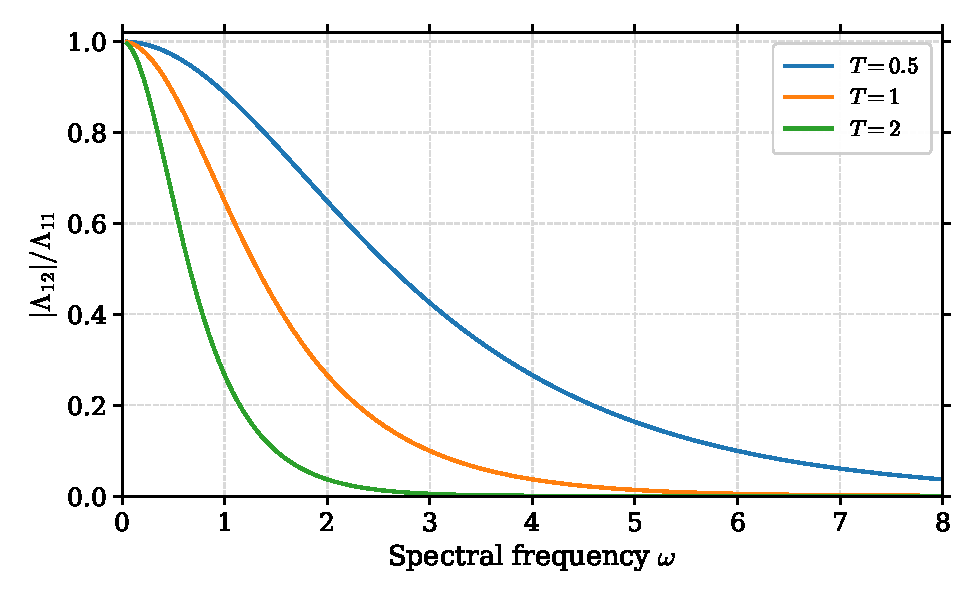
\includegraphics[width=0.77\linewidth]{content/FreeElectronQuantumOptics/figures/geometry-highspin/generated/dn_transmission.pdf}
 \caption{长度为 $T$ 的欧氏振子区间中，Dirichlet-to-Neumann 边界矩阵的跨边界耦合与自耦合之比，精确为 $|\Lambda_{12}|/\Lambda_{11}=1/\cosh(\omega T)$。频率较高或传播区间较长时，边界耦合指数减弱。}
 \label{fig:ghs-dn-transmission}
\end{figure}


令区域 $U_1,U_2$ 沿内部截面 $\Sigma$ 拼接。设各自边界二次型的块矩阵为
\[
 \Lambda_1=\begin{pmatrix}A&B\\B^*&C\end{pmatrix},
 \qquad \Lambda_2=\begin{pmatrix}D&E\\E^*&F\end{pmatrix}.
\]
三个变量分别记为 $f$（左外边界）、$z$（公共内部边界）、$g$（右外边界）。总壳上二次型是
\[
 2\mathscr I=\langle f,Af\rangle+2\operatorname{Re}\langle f,Bz\rangle
 +\langle z,(C+D)z\rangle+2\operatorname{Re}\langle z,Eg\rangle+\langle g,Fg\rangle.
\]
若 $C+D$ 有有界逆，固定外边界条件下对 $z$ 取变分得
$z_*=-(C+D)^{-1}(B^*f+Eg)$。将它代回，新的边界矩阵为
\begin{equation}\label{eq:ghs-dn-schur-complement}
 \Lambda_{U_2\circ U_1}=
 \begin{pmatrix}
 A-B(C+D)^{-1}B^*&-B(C+D)^{-1}E\\
 -E^*(C+D)^{-1}B^*&F-E^*(C+D)^{-1}E
 \end{pmatrix}.
\end{equation}
这就是 Schur 补，而不是另一种新的物理假设。有限维高斯积分还给出行列式因子 $(\det(C+D))^{-1/2}$；连续场论须对该形式行列式做恰当正则化并检查局部边界反项。



令 $U_1$ 为长度 $T_1$ 的区间、$U_2$ 为长度 $T_2$ 的区间。由 \cref{eq:ghs-dn-oscillator-matrix}，
\[
 A=C=\omega\coth\omega T_1,
 \quad B=-\omega\operatorname{csch}\omega T_1,
 \quad D=F=\omega\coth\omega T_2,
 \quad E=-\omega\operatorname{csch}\omega T_2.
\]
Schur 补的左右耦合项为
\[
 -\frac{BE}{C+D}=-\frac{\omega\operatorname{csch}(\omega T_1)
 \operatorname{csch}(\omega T_2)}{\coth(\omega T_1)+\coth(\omega T_2)}.
\]
利用 $\coth a+\coth b=\sinh(a+b)/(\sinh a\sinh b)$，得
$-BE/(C+D)=-\omega\operatorname{csch}[\omega(T_1+T_2)]$。同样利用双曲函数恒等式计算左、右对角项，均得 $\omega\coth[\omega(T_1+T_2)]$。于是 \cref{eq:ghs-dn-schur-complement} 精确恢复 $\Lambda_{T_1+T_2}$，与 \cref{eq:ghs-gluing-kernels} 一致。



这一整套技术只需要正则边界、指定的椭圆问题与可逆性条件，具有比球面径向分解更强的几何普适性。真正的量子泛函积分核是否正定、能否重建 Hilbert 空间，则由反射正性和测度构造决定，不能仅从 Schur 补代数推出。








欧氏理论中的热核从正算子 $A$ 构造，参数 $t$ 越大，高频模态越被压低。但真实时间中的自由场不能按同样的指数衰减演化：自由场的经典演化必须保持初始数据的辛形式，量子理论则由这一辛形式决定正则对易关系。为了弄清哪部分结构真正适用于弯曲时空，需要从 柯西问题出发。


\section{柯西问题}
\label{sec:ghs-cauchy-problem}


设 $(\mathcal M,g_L)$ 是连通、定向并有时间定向的 $d$ 维 Lorentz 流形，度规号差取 $(+,-,\ldots,-)$，时空坐标 $x^0=ct$。一个超曲面 $\Sigma$ 称为 柯西面，如果每条不可延拓类时曲线恰与其相交一次。存在 柯西面并满足通常的因果条件的时空称为全局双曲时空。这个条件的意义不是形式上的便利，而是保证给定初始场与法向导数之后，双曲方程能够得到唯一的全局解。

\begin{theorem}[全局双曲时空的几何分解]
\label{thm:ghs-globally-hyperbolic-splitting}
若 $\mathcal M$ 全局双曲，则存在光滑的 Cauchy 长度时间函数 $x^0$，使 $\mathcal M$ 微分同胚于 $\RR\times\Sigma$，并可写成
\begin{equation}\label{eq:ghs-lorentzian-splitting}
 \mathbf g=\beta(x^0,y)\dd (x^0)^2-h_{x^0},
 \qquad\beta(x^0,y)>0,
\end{equation}
其中每个 $h_{x^0}$ 为 Cauchy 截面上的黎曼度规。这个结论不要求存在任何时间平移 Killing 场。
\end{theorem}

这里引用的是全局双曲时空分解定理；其严格证明使用因果理论与光滑时间函数的构造，不能仅由局部坐标矩阵分解推出。它所带来的关键信息是：Cauchy 发展问题有自然的时间层，却不保证存在真空能量本征态。

\begin{definition}[正则双曲标量算子]
固定质量参数 $\mu=mc/\hbar$ 和曲率耦合 $\xi\in\RR$，定义
\begin{equation}\label{eq:ghs-r6-lorentz-kg-operator}
P=\Box_{g_L}+\mu^2-\xi\mathcal R_L,
\qquad \Box_{g_L}=g_L^{ab}\nabla_a\nabla_b.
\end{equation}
$P\phi=0$ 是实 Klein--Gordon 方程。这里 $\mathcal R_L$ 是 $g_L$ 的标量曲率，$\phi$ 的整体归一化须由作用量或等时对易关系指定；微分方程本身不确定它。
\end{definition}

在平直时空，令 $\phi=\ee^{-\ii\omega t+\ii\vb k\cdot\vb x}$，则 $\Box=c^{-2}\partial_t^2-\Delta$，因而 $P\phi=0$ 等价于
\[
\omega^2=c^2|\vb k|^2+\frac{m^2c^4}{\hbar^2},
\qquad E=\hbar\omega=\sqrt{\hbar^2c^2|\vb k|^2+m^2c^4}.
\]
平面波代入给出 $-\omega^2/c^2+|\vb k|^2+\mu^2=0$，同时固定了质量项与正频号差；曲率耦合的符号由下列作用量固定。

\begin{figure}[htbp]
\centering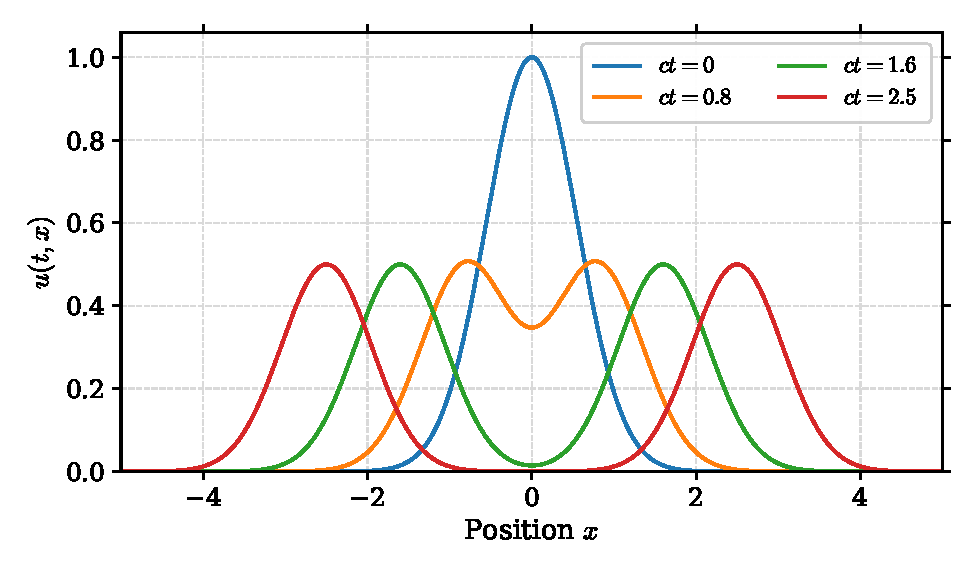
\includegraphics[width=.79\linewidth]{content/FreeElectronQuantumOptics/figures/geometry-highspin/generated/cauchy_wave_packets.pdf}
\caption{一维无质量波动方程 $u_{tt}=c^2u_{xx}$ 的精确达朗贝尔解：初始高斯位移、初始速度为零时，波包向左右以速度 $c$ 分离。横轴采用相同的长度单位。}\label{fig:ghs-cauchy-wave-packets}
\end{figure}

\cref{fig:ghs-cauchy-wave-packets} 对应 $u(t,x)=[f(x-ct)+f(x+ct)]/2$，它展示的是 Cauchy 初值的因果传播，而不是把某个静态本征模简单作衰减演化。

\begin{theorem}[双曲 柯西问题]\label{thm:ghs-r6-cauchy-wellposed}
在光滑全局双曲时空上，对于光滑紧支 柯西初始数据 $(f,p)$ 和适当紧支源 $j$，$P\phi=j$ 有唯一光滑解，并满足有限传播速度；解在任意 柯西面的支持包含在初始数据与源支持的因果传播集合之中。
\end{theorem}
这个定理依赖一般双曲算子的能量估计与全局双曲性。我们在下面证明其中的守恒量及其在量子化中的意义；定理的完整全局存在性证明属于双曲偏微分方程理论，不能用一组平面波代替。相关数学背景可参见 \cite{ghs-r6-baer-wave}。

\begin{figure}[htbp]
\centering
% Local TikZ geometry; styles inherited exclusively from the shared preamble.
\begin{tikzfig}[scale=.95]
\draw[lecturearrow] (-3,0)--(3,0) node[right] {$x$};
\draw[lecturearrow] (0,-.45)--(0,3.65) node[above] {$ct$};
\fill[blue!7] (0,0)--(-3,3)--(3,3)--cycle;
\draw[thick] (0,0)--(-3,3) (0,0)--(3,3);
\draw[gray,dashed] (-3,3)--(3,3);
\draw[thick,blue!70!black] (-2.8,.85)--(2.8,.85);
\draw[thick,red!70!black] (-2.8,2.13)--(2.8,2.13);
\node[lecturelabel] at (-2.6,1.12) {$\Sigma_0$};
\node[lecturelabel] at (2.6,2.42) {$\Sigma_1$};
\node[lecturelabel] at (2.7,3.32) {Null rays};
\fill (0,0) circle (1.6pt);
\end{tikzfig}

\caption{平直 $1+1$ 时空中的未来光锥与两张时间切片示意。斜线是光速特征线；有限传播速度约束的是扰动的支持，而不是对振幅作欧氏热核式的指数衰减。}\label{fig:ghs-causal-domain}
\end{figure}

\cref{fig:ghs-causal-domain} 只用于展示局部因果锥。一般弯曲时空上的 柯西面不必是图中的直线，且全局双曲性的证明仍须使用时空的整体因果结构。


为避免将场的量纲归一化混入几何计算，可把实场 $\phi$ 规范化为长度维数 $L^{(2-d)/2}$，并取
\begin{equation}\label{eq:ghs-r6-kg-action}
S[\phi]=\frac{\hbar}{2}\int_{\mathcal M}
\left(g_L^{ab}\nabla_a\phi\nabla_b\phi-(\mu^2-\xi\mathcal R_L)\phi^2\right)\dd\mu_{g_L}.
\end{equation}
积分使用 $x^0=ct$ 的长度测度，因此整体具有作用量量纲。在坐标体积测度 $\dd\mu_{g_L}=\sqrt{|\det g_L|}\dd^dx$ 下，分部积分给出
\begin{align*}
\delta S
&=\hbar\int_{\mathcal M}\left(\nabla^a\phi\nabla_a\delta\phi-(\mu^2-\xi\mathcal R_L)\phi\delta\phi\right)\dd\mu_{g_L}\\
&=-\hbar\int_{\mathcal M}(P\phi)\delta\phi\dd\mu_{g_L}
 +\hbar\int_{\partial\mathcal M}\nabla^a\phi\delta\phi\dd\Sigma_a.
\end{align*}
$\dd\Sigma_a$ 是有向面元；在两张类空面围成的区域，未来面的面元为 $+n_a\dd\mu_\Sigma$，过去面为 $-n_a\dd\mu_\Sigma$，其中 $n^an_a=+1$。固定边界场消去最后一项，得到 $P\phi=0$；未来面的动量密度为 $\hbar n^a\nabla_a\phi$。

\begin{proposition}[解空间上的守恒辛流]\label{prop:ghs-r6-symplectic-current}
对两个实解 $\phi_1,\phi_2$，定义
\begin{equation}\label{eq:ghs-r6-current}
j^a(\phi_1,\phi_2)=\phi_1\nabla^a\phi_2-\phi_2\nabla^a\phi_1.
\end{equation}
如果两解满足同一个实势 $P\phi_i=0$，则 $\nabla_aj^a=0$。对具有合适空间支撑的解，
\begin{equation}\label{eq:ghs-r6-covariant-symplectic}
\sigma_\Sigma(\phi_1,\phi_2)=\int_\Sigma n_aj^a(\phi_1,\phi_2)\dd\mu_\Sigma
\end{equation}
与 柯西面的选择无关；其整体乘以 $\hbar$ 就是作用量 \cref{eq:ghs-r6-kg-action} 对应的物理辛形式。
\end{proposition}
\begin{proof}
对流取散度，乘法法则给出
\begin{align*}
\nabla_aj^a&=(\nabla_a\phi_1)(\nabla^a\phi_2)+\phi_1\Box\phi_2
 -(\nabla_a\phi_2)(\nabla^a\phi_1)-\phi_2\Box\phi_1\\
&=\phi_1(\Box\phi_2)-\phi_2(\Box\phi_1).
\end{align*}
将 $\Box\phi_i=-(\mu^2-\xi\mathcal R_L)\phi_i$ 代入，两个势项抵消，散度为零。让 $\Sigma_1,\Sigma_2$ 围成一个紧致截断时空区域，应用 Lorentz 型散度定理：两张 柯西面的通量之差等于侧边界通量与体积分。取空间紧支解时，可以选取侧边界在因果传播之外，侧边界通量为零，所以两个 柯西面上的通量相等。一般非紧支情形还需指定足以消去无穷远通量的衰减条件。
\end{proof}

未来单位法向满足 $n_an^a=+1$。在超静态度规 $g_L=c^2\dd t^2-h$ 上，$n^a\nabla_a=c^{-1}\partial_t$，所以
\[
 \sigma_\Sigma(\phi_1,\phi_2)=\frac1c\int_\Sigma
 (\phi_1\partial_t\phi_2-\phi_2\partial_t\phi_1)\dd\mu_h.
\]
这个因子由长度坐标而来；$\hbar\sigma$ 是有作用量量纲的物理辛形式。

柯西解具有唯一性后，可以将任意外源分解为许多局部扰动，再由对每个源都适用的 Green 算子恢复整体解。因果支持条件将在这里取代欧氏核的衰减条件。


在全局双曲条件下存在先进和延迟 Green 算子 $G_{\mathrm A},G_{\mathrm R}$，满足
\begin{equation}\label{eq:ghs-r6-causal-green}
PG_{\mathrm R}f=PG_{\mathrm A}f=f,
\qquad\operatorname{supp}(G_{\mathrm R}f)\subset J^+(\operatorname{supp}f),
\quad\operatorname{supp}(G_{\mathrm A}f)\subset J^-(\operatorname{supp}f).
\end{equation}
初值为零的受迫解用 $G_{\mathrm R}$ 表示；其源只能影响未来，因此支持条件本身承载因果性。定义 $E=G_{\mathrm R}-G_{\mathrm A}$，则 $PEf=0$。这里 $E$ 是因果传播算子，既不是欧氏椭圆 Green 算子，也不是 Feynman 传播子。

\begin{proposition}[因果传播与辛配对]\label{prop:ghs-r6-causal-pairing}
取 $f,h\in C_c^\infty(\mathcal M)$，令 $Ef,Eh$ 是相应的空间紧支解。按 \cref{eq:ghs-r6-covariant-symplectic} 的约定，可将源与解的配对归约为
\begin{equation}\label{eq:ghs-r6-peierls}
\sigma(Ef,Eh)=-\int_{\mathcal M}f(x)(Eh)(x)\dd\mu_{g_L}(x),
\end{equation}
其中 $E=G_{\mathrm R}-G_{\mathrm A}$、未来法向以及 $P$ 均已固定，负号由 Green 恒等式确定。
\end{proposition}
\begin{proof}
令 $\Sigma_+$ 位于 $\operatorname{supp}f\cup\operatorname{supp}h$ 的未来。$G_{\mathrm R}f$ 在足够早的 柯西面上为零，并在 $\Sigma_+$ 上与 $Ef$ 具有相同数据。对满足 $P\psi=0$ 的 $\psi=Eh$，计算
\[
\nabla_aj^a(G_{\mathrm R}f,\psi)
=(G_{\mathrm R}f)P\psi-\psi P(G_{\mathrm R}f)=-f\psi.
\]
将其在一张过去 柯西面与 $\Sigma_+$ 之间积分。过去通量为零，未来有向面元为 $+n_a\dd\mu_\Sigma$，故
\[
 \sigma(Ef,Eh)=\int\nabla_aj^a\dd\mu_{g_L}=-\int f(Eh)\dd\mu_{g_L}.
\]
源函数的自由场取 $\widehat\phi(f)=\widehat\Phi(Ef)$，于是 $[\widehat\phi(f),\widehat\phi(h)]=-\ii\int f(Eh)\dd\mu_{g_L}$。可以用单模直接核对：$P_\omega=\partial_0^2+\omega^2$ 的因果核为 $E_\omega(s)=\sin(\omega s)/\omega$，正频二点函数 $W_\omega(s)=\ee^{-\ii\omega s}/(2\omega)$ 满足 $W_\omega(s)-W_\omega(-s)=-\ii E_\omega(s)$。反对称部分与正频模归一化因而一致。
\end{proof}


经典解空间中的 $\sigma$ 是反对称双线性形式。量子理论将其编码为酉算符 $W(u)$ 的乘法规则
\begin{equation}\label{eq:ghs-r6-weyl-algebra}
W(u)W(v)=\exp\!\left[-\frac{\ii}{2}\sigma(u,v)\right]W(u+v),
\qquad W(u)^*=W(-u).
\end{equation}
这里 $u,v$ 可视为归一化量纲下的经典解，采用 $W(u)=\ee^{\ii\widehat\Phi(u)}$，因此由 Baker--Campbell--Hausdorff 公式可知 $[\widehat\Phi(u),\widehat\Phi(v)]=\ii\sigma(u,v)\id$。在有量纲的正则坐标 $(q,p)$ 上，直接使用 $[\widehat q,\widehat p]=\ii\hbar\id$；这与作用量的 $\hbar$ 规范化一致，而不是把 SI 常数设为一。



辛形式在演化中守恒，使 Weyl 算符的乘法相位保持不变。

\begin{proposition}[辛变换诱导场代数自同构]
\label{prop:ghs-r6-symplectic-automorphism}
若线性映射 $T$ 保持 $\sigma$，即 $\sigma(Tu,Tv)=\sigma(u,v)$，则 $W(u)\mapsto W(Tu)$ 保持 Weyl 乘法及伴随，因而定义 Weyl 代数的自同构。它未必由选定 Fock 空间中的一个酉算符实现。
\end{proposition}

\begin{proof}
将 $W(Tu)W(Tv)$ 用 \cref{eq:ghs-r6-weyl-algebra} 展开，并利用 $\sigma(Tu,Tv)=\sigma(u,v)$ 及 $T(u+v)=Tu+Tv$，得到原来的乘法相位。又因 $T(-u)=-Tu$，伴随也保持。此证明完全发生在抽象代数上，没有使用某一个真空表示，所以不能从它推断特定 Hilbert 空间中必然存在实现 $T$ 的酉算符。
\end{proof}

这就是为何一般时空量子场论首先需要可在不同曲率背景上定义的算符代数，再进一步选择量子态。平直空间的正频真空是一个非常重要的选择，却不是全局双曲性自动赠送的唯一结构。


因果传播的反对称部分决定经典解的辛配对。量子化时，辛配对不需要先选择任何真空，就已经能够确定正则对易代数。


在一般全局双曲时空中，场的正频划分依赖量子态；但在超静态背景 $g_L=c^2\dd t^2-h_{ij}(x)\dd x^i\dd x^j$ 上，若 $h$ 与 $t$ 无关，空间算子
\[
A=-\Delta_h+\mu^2+\xi\mathcal R_h
\]
自伴且满足 $A\ge m_0^2>0$。由于 $\mathcal R_L=-\mathcal R_h$，$P=c^{-2}\partial_t^2+A$，则波动方程等价于 $\partial_t^2\phi+c^2A\phi=0$。以 $\Omega=c\sqrt A$ 定义频率算子，利用谱演算便可写下不要求离散本征函数的精确 柯西解
\begin{equation}\label{eq:ghs-r6-ultrastatic-exact-flow}
\phi(t)=\cos(t\Omega)f+\Omega^{-1}\sin(t\Omega)p,
\qquad p=\partial_t\phi(0).
\end{equation}
其中 $f\in\operatorname{Dom}(A^{1/2})$、$p\in L^2(\Sigma)$ 为有限能量数据。

将初始位置和速度记为列向量 $X_0=(f,p)^{\mathsf T}$。由解析解再求一次时间导数，得到整个经典演化的块算子矩阵
\begin{equation}\label{eq:ghs-r12-ultrastatic-symplectic-matrix}
 X_t=\begin{pmatrix}
 C_t&\Omega^{-1}S_t\\
 -\Omega S_t&C_t
 \end{pmatrix}X_0,\qquad
 C_t=\cos(t\Omega),\quad S_t=\sin(t\Omega).
\end{equation}
这些算子都是 $\Omega$ 的实函数，因而两两对易且在共同定义域上满足 $C_t^2+S_t^2=I$。对两组有限能量初值 $X=(f,p)$、$Y=(g,q)$，定义实辛形式
\[
 \sigma(X,Y)=c^{-1}\bigl(\langle f,q\rangle_{L^2}-\langle p,g\rangle_{L^2}\bigr).
\]
用 \cref{eq:ghs-r12-ultrastatic-symplectic-matrix} 展开 $\sigma(X_t,Y_t)$，含 $C_tS_t$ 的交叉项因自伴性而抵消，含 $C_t^2$、$S_t^2$ 的两组项相加回到 $\sigma(X,Y)$。这给出了演化保持辛形式的一个直接证明，并说明保辛条件并不依赖是否能够把谱写成离散求和。需要说明的是，$\Omega S_t$ 在 $L^2$ 上通常无界；矩阵公式应理解为从有限能量数据空间 $\operatorname{Dom}(\Omega)\oplus L^2$ 到自身的连续演化，而不是把每个块都当作 $L^2$ 上的有界算子。

两个算子函数有界并强连续；因此此表达对存在连续谱的截面同样成立，无须写出“求和所有球谐”的假设。

\begin{proposition}[有限能量及辛量的守恒]
对上述静态方程，定义能量范数（物理场能量为 $\hbar\mathcal E/c$）
\begin{equation}\label{eq:ghs-r6-ultrastatic-energy}
\mathcal E(t)=\frac12\left(\norm{\partial_t\phi(t)}_{L^2}^2
+c^2\norm{A^{1/2}\phi(t)}_{L^2}^2\right).
\end{equation}
对适当光滑数据，$\mathcal E(t)$ 与 $t$ 无关；同时两组解的 柯西数据辛积
$c^{-1}\int_\Sigma(\phi_1\partial_t\phi_2-\partial_t\phi_1\phi_2)\dd\mu_h$ 守恒。
\end{proposition}
\begin{proof}
对能量求导，利用 $A$ 自伴与方程得
\begin{align*}
\mathcal E'(t)
&=\langle\partial_t\phi,\partial_t^2\phi\rangle
+c^2\langle A^{1/2}\phi,A^{1/2}\partial_t\phi\rangle\\
&=\langle\partial_t\phi,-c^2A\phi\rangle
+c^2\langle A\phi,\partial_t\phi\rangle=0.
\end{align*}
若 $\phi_1,\phi_2$ 分别为解，则辛积的导数是
\[
\int_\Sigma(\phi_1\partial_t^2\phi_2-\partial_t^2\phi_1\phi_2)\dd\mu_h
=-c^2\bigl(\langle\phi_1,A\phi_2\rangle-\langle A\phi_1,\phi_2\rangle\bigr)=0.
\]
此处先对实解作计算；复解使用相应共轭内积。由光滑有限谱近似可将恒等式推广到有限能量解。
\end{proof}

若 $A$ 具有正交本征函数 $u_j$、$Au_j=\lambda_ju_j$，设 $\omega_j=c\sqrt{\lambda_j}$，则 \cref{eq:ghs-r6-ultrastatic-exact-flow} 逐模给出
\[
q_j(t)=f_j\cos(\omega_jt)+\frac{p_j}{\omega_j}\sin(\omega_jt).
\]
但它只是谱演算在离散谱下的表示，并不是更一般形式的推导依据。若 $A$ 有零模，$\sin(t\Omega)/\Omega$ 在该谱子空间的连续极限为 $t$，零模发生线性时间漂移；若 $A$ 有负谱，$\sqrt A$ 不再是正自伴频率算子，相应模态产生指数增长，不能照用正频真空。


当 $A\ge m_0^2>0$ 时，$\ee^{-\tau\Omega}$ 对 $\tau\ge0$ 是收缩半群。若物理真空确实选取正频的静态谱分解，二点函数的正时间差部分由谱测度给出
\begin{equation}\label{eq:ghs-r6-ultrastatic-twopoint}
W(t,x;t',y)=\int_{(0,\infty)}
\frac{\ee^{-\ii c\sqrt\lambda(t-t')}}{2\sqrt\lambda}
\dd\mathsf E_A(\lambda)(x,y),
\end{equation}
其中采用正文归一化场的长度坐标 $x^0=ct$；若改用物理时间作为共轭 Cauchy 变量，整体归一化因子需一并换算。上式按分布意义理解，并须排除不受控的零谱贡献。将 $c(t-t')$ 在适当解析域继续为 $-\ii\tau$，可得到含 $\ee^{-\tau\sqrt A}/(2\sqrt A)$ 的欧氏核。

然而这一 Wick 延拓使用了静态正频分解及谱正性。一般随时间改变的空间没有同一个 $\Omega$ 对角化所有时间演化，更不保证存在全局解析的虚时间方向。因此“欧氏泛函积分等于 Lorentz 量子态”的陈述必须附带反射正性、解析延拓和所选量子态的条件，而不能作为任意时空的定义。


\section{复结构与正频}
\label{sec:ghs-complex-structure-frequency}


设 $V$ 是 $2N$ 维实向量空间，$\sigma:V\times V\to\RR$ 非退化且反对称。线性算子 $J:V\to V$ 若满足 $J^2=-\id$、$\sigma(Ju,Jv)=\sigma(u,v)$，就使 $V$ 成为一个复向量空间，其中虚数单位以 $J$ 表示。为使量子一粒子内积正定，还要求
\begin{equation}\label{eq:ghs-r6-compatible-J}
g_J(u,v):=\sigma(u,Jv)
\quad\text{为对称正定双线性型}.
\end{equation}

\begin{proposition}[从辛结构构造一粒子内积]
若 $J$ 满足上述条件，在复向量空间 $(V,J)$ 上定义
\begin{equation}\label{eq:ghs-r6-oneparticle-inner}
\langle u,v\rangle_J=\frac12g_J(u,v)+\frac{\ii}{2}\sigma(u,v).
\end{equation}
按第一个变量共轭线性、第二个变量线性的约定，它是正定 Hermite 内积。
\end{proposition}
\begin{proof}
由 $\sigma(Ju,Jv)=\sigma(u,v)$ 和 $J^2=-\id$ 可得 $\sigma(Ju,v)=-\sigma(u,Jv)$，所以
$g_J(v,u)=\sigma(v,Ju)=-\sigma(Ju,v)=\sigma(u,Jv)=g_J(u,v)$。
再算复线性：
\begin{align*}
\langle u,Jv\rangle_J
&=\tfrac12\sigma(u,J(Jv))+\tfrac{\ii}{2}\sigma(u,Jv)\\
&=-\tfrac12\sigma(u,v)+\tfrac{\ii}{2}g_J(u,v)
=\ii\langle u,v\rangle_J.
\end{align*}
交换两个变量并复共轭，反对称性保证 $\langle v,u\rangle_J=\overline{\langle u,v\rangle_J}$。最后 $\langle u,u\rangle_J=g_J(u,u)/2>0$。因此得到真正的复 Hilbert 内积，而不仅是一个形式上的频率分解。
\end{proof}


\begin{figure}[htbp]
\centering
% Local TikZ geometry; styles inherited exclusively from the shared preamble.
\begin{tikzfig}[scale=.93]
\draw[lecturearrow,gray!80] (-3.8,0)--(-.25,0) node[right] {$q$};
\draw[lecturearrow,gray!80] (-2,-1.8)--(-2,1.8) node[above] {$p$};
\draw[thick,blue!65!black] (-2,0) circle (1.1);
\draw[lecturearrow,gray!80] (.15,0)--(4.65,0) node[right] {$q$};
\draw[lecturearrow,gray!80] (2.4,-1.8)--(2.4,1.8) node[above] {$p$};
\draw[thick,red!65!black] (2.4,0) ellipse (1.84 and .6576);
\node[lecturelabel] at (-2,-2.25) {Unsqueezed};
\node[lecturelabel] at (2.4,-2.25) {Squeezed};
\node[lecturelabel] at (.25,2.1) {$\det \sigma=\mathrm{constant}$};
\end{tikzfig}

\caption{相空间中的两种等面积高斯协方差椭圆。单模压缩通过辛变换拉长 $q$ 向、压短 $p$ 向，但纯态的不确定度面积（$\det\sigma$）不变。}\label{fig:ghs-squeezed-symplectic}
\end{figure}

\cref{fig:ghs-squeezed-symplectic} 区分了“真空态的选择”和“真实粒子数变化”：只改变正频分解也可改变 高斯椭圆的观察方式，但它仍必须满足辛相容性。

\subsection{复结构选择与有限模高斯态}

对质量已吸收到 $q,p$ 的谐振子，取
\begin{equation}\label{eq:ghs-r6-oscillator-H}
H_\omega(q,p)=\frac12(p^2+\omega^2q^2),\qquad
\sigma((q,p),(q',p'))=qp'-pq'.
\end{equation}
它的 Hamilton 流满足 $\dot q=p,\ \dot p=-\omega^2q$。与其相容的一个正复结构是
\begin{equation}\label{eq:ghs-r6-oscillator-J}
J_\omega(q,p)=\left(-\frac p\omega,\omega q\right).
\end{equation}
验证 $J_\omega^2=-\id$ 不需要额外假设；再直接计算
\[
\sigma((q,p),J_\omega(q,p))=\omega q^2+\frac{p^2}{\omega}>0
\quad((q,p)\ne0).
\]
从 $J_\omega$ 出发，在量子代数 $[\widehat q,\widehat p]=\ii\hbar$ 下定义
\begin{equation}\label{eq:ghs-oscillator-annihilator-general}
 a_\omega=\sqrt{\frac{\omega}{2\hbar}}\,\widehat q
 +\frac{\ii}{\sqrt{2\hbar\omega}}\,\widehat p,
\quad
 a_\omega^\dagger=\sqrt{\frac{\omega}{2\hbar}}\,\widehat q
 -\frac{\ii}{\sqrt{2\hbar\omega}}\,\widehat p.
\end{equation}
直接代入可得 $[a_\omega,a_\omega^\dagger]=1$，同时
\begin{equation}\label{eq:ghs-r6-oscillator-number}
\widehat H_\omega=\hbar\omega\left(a_\omega^\dagger a_\omega+\frac12\right).
\end{equation}
这里能量量纲和零点能都保留了 $\hbar$，所以频率选取不是单纯的记号问题。

\begin{theorem}[一个模态的真空波函数]
在 $q$ 表象中，$a_\omega\psi_0=0$ 的归一化解为
\begin{equation}\label{eq:ghs-r6-gaussian-vacuum}
\psi_{0,\omega}(q)=\left(\frac{\omega}{\pi\hbar}\right)^{1/4}
\exp\left(-\frac{\omega q^2}{2\hbar}\right).
\end{equation}
且 $\langle q^2\rangle=\hbar/(2\omega)$、$\langle p^2\rangle=\hbar\omega/2$。
\end{theorem}
\begin{proof}
在坐标表示 $\widehat p=-\ii\hbar\partial_q$，所以 $a_\omega\psi_0=0$ 等价于
\[
\left(\sqrt{\omega}\,q+\frac{\hbar}{\sqrt\omega}\partial_q\right)\psi_0=0,
\qquad\frac{\psi'_0}{\psi_0}=-\frac{\omega}{\hbar}q.
\]
积分给出 $\psi_0=C\exp[-\omega q^2/(2\hbar)]$，用 高斯积分 $\int_\RR\exp(-\omega q^2/\hbar)\dd q=\sqrt{\pi\hbar/\omega}$ 得到系数。对 $|\psi_0|^2$ 求二阶矩给第一个方差；动量二阶矩可由 $p\psi_0=\ii\omega q\psi_0$ 得到。所有结果都可从正则对易关系独立核对。
\end{proof}


将 $N$ 个坐标与动量排列成列向量 $X=(q_1,\ldots,q_N,p_1,\ldots,p_N)^{\mathsf T}$，令
\[
\mathbb J=\begin{pmatrix}0&I_N\\-I_N&0\end{pmatrix},
\qquad [\widehat X_a,\widehat X_b]=\ii\hbar\mathbb J_{ab}.
\]
对零均值量子态，协方差矩阵是实对称矩阵
\begin{equation}\label{eq:ghs-r6-covariance}
V_{ab}=\frac12\langle\widehat X_a\widehat X_b+
\widehat X_b\widehat X_a\rangle.
\end{equation}
把非负算符 $\langle(\sum z_a\widehat X_a)^\dagger(\sum z_b\widehat X_b)\rangle$ 展开，得到 Robertson--Schrödinger 不等式
\begin{equation}\label{eq:ghs-r6-gaussian-uncertainty}
V+\frac{\ii\hbar}{2}\mathbb J\ge0.
\end{equation}
其中“$\ge0$”表示左边 Hermite 矩阵半正定，而不是要求其全部元素非负。对于一个模态，取 $V=\begin{psmallmatrix}a&c\\c&b\end{psmallmatrix}$，主子式条件给出
\[
a\ge0,\qquad ab-c^2\ge\hbar^2/4.
\]
这比分别使用 $\Delta q\Delta p\ge\hbar/2$ 更强，因为它还包含关联项 $c$。



在正则变量作线性辛变换后，协方差也相应改变，而正则对易关系与不确定关系保持不变。

若实矩阵 $S$ 满足 $S\mathbb J S^{\mathsf T}=\mathbb J$，则 $X'=SX$ 保持正则对易关系，协方差变为 $V'=SVS^{\mathsf T}$，并保持不等式 \cref{eq:ghs-r6-gaussian-uncertainty}。

对易子矩阵变换为 $[X'_a,X'_b]=\ii\hbar(S\mathbb JS^{\mathsf T})_{ab}$，由辛条件等于原矩阵。由于
\[
V'+\frac{\ii\hbar}2\mathbb J
=S\left(V+\frac{\ii\hbar}2\mathbb J\right)S^{\mathsf T},
\]
任意向量 $z$ 的二次型等于 $S^{\mathsf T}z$ 对原非负矩阵的二次型，故仍非负。




\subsection{Bogoliubov 变换与粒子产生}

两个正复结构 $J_0,J_1$ 定义不同的湮灭算符。对离散模态写最一般保持正则对易关系的线性关系
\begin{equation}\label{eq:ghs-r6-bogoliubov-matrix}
b_i=\sum_j\left(\alpha_{ij}a_j+\beta_{ij}a_j^\dagger\right).
\end{equation}
不能独立任选 $\alpha,\beta$：分别算 $[b_i,b_j^\dagger]$ 和 $[b_i,b_j]$，得到
\begin{equation}\label{eq:ghs-r6-bogoliubov-identities}
\alpha\alpha^\dagger-\beta\beta^\dagger=I,
\qquad \alpha\beta^{\mathsf T}=\beta\alpha^{\mathsf T}.
\end{equation}
其中第一式的负号来自 $[a_i^\dagger,a_j]=-\delta_{ij}$，第二式来自两个湮灭算符必须对易。

\begin{theorem}[两种真空的粒子数]\label{thm:ghs-r6-bogoliubov-number}
若 $a_j|0_a\rangle=0$，且变换 \cref{eq:ghs-r6-bogoliubov-matrix} 在所讨论的 Fock 表示中有意义，则
\begin{equation}\label{eq:ghs-r6-created-particles}
\langle0_a|b_i^\dagger b_i|0_a\rangle=\sum_j|\beta_{ij}|^2,
\qquad \langle0_a|N_b|0_a\rangle=\operatorname{Tr}(\beta\beta^\dagger).
\end{equation}
对于无限维单粒子空间，有限的总粒子数要求 $\beta$ 为 Hilbert--Schmidt 算子；它也正是通常 Shale--Stinespring 酉实现判据的条件。
\end{theorem}
\begin{proof}
将 $b_i^\dagger b_i$ 展开为 $a^\dagger a$、$a^\dagger a^\dagger$、$aa$、$aa^\dagger$ 四类项。前三类在 $a$ 真空的期望值均为零，只有
\[
\sum_{j,k}\overline{\beta_{ij}}\beta_{ik}\langle0_a|a_ja_k^\dagger|0_a\rangle
=\sum_j|\beta_{ij}|^2
\]
保留。再对 $i$ 求和即得迹公式。无限维情况下上式可能发散；代数变换合法不等于必然在同一个 Fock 空间中可酉实现。Hilbert--Schmidt 判据作为无限维表示定理调用 \cite{ghs-r6-shale}，不能从有限维迹恒等式单独推出。
\end{proof}


例如，在频率突然改变的计算中，
谐振子由频率 $\omega_0>0$ 突然变为 $\omega_1>0$，$q,p$ 在改变瞬间连续。把两套 $a_\omega$ 的定义相互代入，得到
\begin{equation}\label{eq:ghs-sudden-quench-bogoliubov}
\alpha=\frac12\left(\sqrt{\frac{\omega_1}{\omega_0}}+\sqrt{\frac{\omega_0}{\omega_1}}\right),\quad
\beta=\frac12\left(\sqrt{\frac{\omega_1}{\omega_0}}-\sqrt{\frac{\omega_0}{\omega_1}}\right).
\end{equation}
\begin{proof}
由旧频率下的湮灭算符反解
\[
 q=\sqrt{\frac{\hbar}{2\omega_0}}(a_0+a_0^\dagger),\qquad
 p=-\ii\sqrt{\frac{\hbar\omega_0}{2}}(a_0-a_0^\dagger).
\]
代入新频率下的 $a_1$，分别整理两种算符的系数，得到
\begin{align*}
 a_1&=\tfrac12\sqrt{\omega_1/\omega_0}(a_0+a_0^\dagger)
      +\tfrac12\sqrt{\omega_0/\omega_1}(a_0-a_0^\dagger)\\
 &=\alpha a_0+\beta a_0^\dagger.
\end{align*}
$|\alpha|^2-|\beta|^2=1$ 保持正则对易关系，旧真空只有 $\langle a_0a_0^\dagger\rangle=1$ 这一收缩，故新粒子数为 $|\beta|^2$。
\end{proof}

直接展开 $\alpha^2-\beta^2=1$，旧真空在新粒子基下的平均数是
\begin{equation}\label{eq:ghs-r6-quench-number}
\langle N_1\rangle=|\beta|^2
=\frac{(\omega_1-\omega_0)^2}{4\omega_0\omega_1}.
\end{equation}
该结果确切反映两种正频定义的差异；真正的时变时空还必须证明相应模态方程、初始态存在性以及高频绝热行为。


\begin{figure}[htbp]
\centering
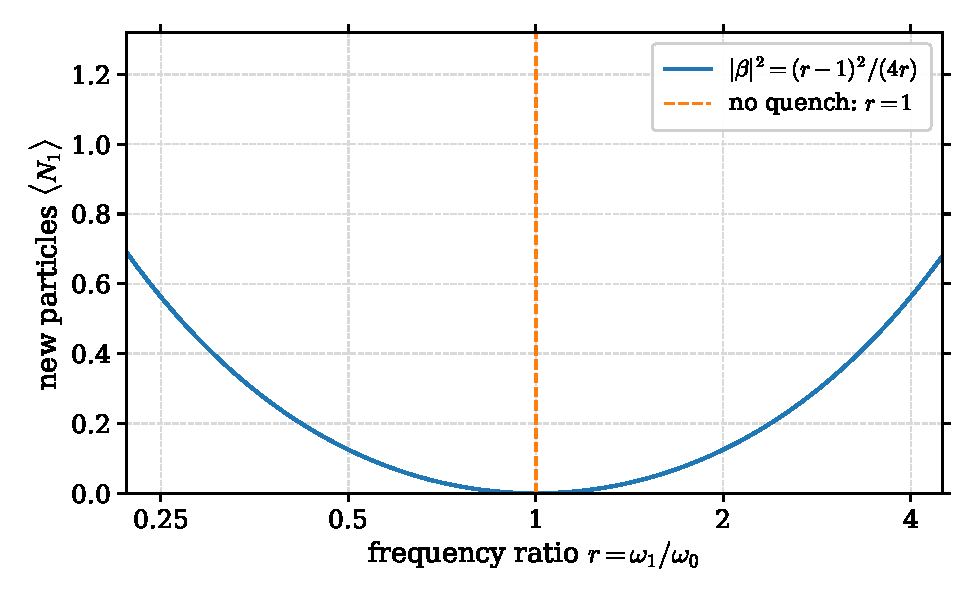
\includegraphics[width=.78\linewidth]{content/FreeElectronQuantumOptics/figures/geometry-highspin/generated/quench_particles.pdf}
\caption{谐振子频率突变时旧真空中的新粒子数，直接取自 \cref{eq:ghs-r6-quench-number}。水平轴使用对数刻度，使 $r\leftrightarrow r^{-1}$ 的精确对称性可见。}
\label{fig:ghs-r6-quench}
\end{figure}


考虑一个规范化的单模玻色代数 $[a,a^\dagger]=1$。固定实数 $r\ge0$，定义
$S(r)=\exp[\tfrac r2(a^2-a^{\dagger 2})]$ 与 $|\psi_r\rangle=S(r)|0\rangle$。
由交换子级数可得 $S(r)aS(r)^\dagger=a\cosh r+a^\dagger\sinh r$，
因此 $|\psi_r\rangle$ 满足 $(a\cosh r+a^\dagger\sinh r)|\psi_r\rangle=0$。
在数态基底中写 $|\psi_r\rangle=\sum_{m\ge0}c_m|m\rangle$，
比较 $|m\rangle$ 的系数便得到递推式
\[
 c_{m+1}\sqrt{m+1}\cosh r+c_{m-1}\sqrt m\sinh r=0,
 \qquad c_{-1}=0.
\]
从 $m=0$ 起，全部奇数系数为零；再对 $m=2n+1$ 递推，得到
$c_{2n}=(-\tanh r)^n\sqrt{(2n)!}\,c_0/(2^nn!)$。
归一化使用 $\sum_{n\ge0}\binom{2n}{n}z^n/4^n=(1-z)^{-1/2}$，
从而 $|c_0|^2=1/\cosh r$。因此准确的数态分布为
\begin{equation}\label{eq:ghs-r8-one-mode-squeezed-parity}
 P_{2n}=\frac{(2n)!}{2^{2n}(n!)^2}\frac{\tanh^{2n}r}{\cosh r},
 \qquad P_{2n+1}=0.
\end{equation}
这和后文双模压缩态的热形约化谱不同：单模真空压缩只占据偶数数态，而双模纯态偏迹后每个非负整数占据数都有非零权重。

\begin{figure}[htbp]
\centering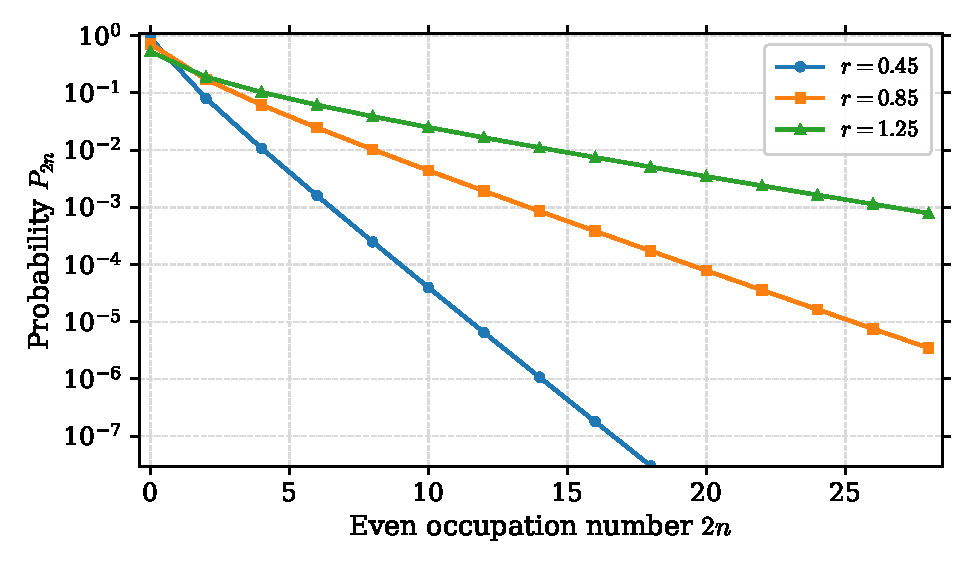
\includegraphics[width=.78\linewidth]{content/FreeElectronQuantumOptics/figures/geometry-highspin/generated/squeezed_even_statistics.pdf}
\caption{单模压缩真空的精确偶数粒子数分布 \cref{eq:ghs-r8-one-mode-squeezed-parity}。横轴只列出偶数态；所有奇数态的概率严格为零。}
\label{fig:ghs-squeezed-even-statistics}
\end{figure}

\cref{fig:ghs-squeezed-even-statistics} 中 $r$ 增大时，分布扩展到更高的偶数数态。峰形变化不是粒子数守恒动力学中的衰变，而是对不同复结构定义的真空作 Fock 基底展开所得。


一个相容复结构选定了正频，也选定了相应的 Fock 真空。不同几何或不同观察者给出的两种复结构未必一致；比较它们时，真正应计算的是正频与负频模的混合。


有限维正则对易代数的不可约正规表示在通常条件下酉等价，因此对有限个谐振子选取新的正频基总可以通过某个 Fock 空间幺正算子实现。对曲时空量子场，无穷多个模态会同时被混合；若忽略极限，就可能把每个有限模态上的合法变换误判为整个量子场的幺正时间演化。这个问题能在\emph{完全对角}的 Bogoliubov 变换中直接算出。

先考虑一列相互独立的规范化玻色模态 $a_j$，$j\in\NN$，满足 $[a_j,a_k^\dagger]=\delta_{jk}$。对每个模态取 $r_j\ge0$，令
\begin{equation}\label{eq:ghs-r7-diagonal-bogoliubov}
 b_j=\cosh r_j\,a_j+\sinh r_j\,a_j^\dagger,
 \qquad \beta_j=\sinh r_j.
\end{equation}
直接使用 $[a_j,a_j^\dagger]=1$ 验证
$[b_j,b_j^\dagger]=\cosh^2r_j-\sinh^2r_j=1$。对有限个模态，它总能由压缩幺正算子实现。设 $|0_j\rangle$ 是 $a_j$ 真空，寻找满足 $b_j|\Omega_j\rangle=0$ 的归一态。由于 $b_j$ 只连接相差两个量子数的数态，可以取偶数展开
\[
 |\Omega_j\rangle=\sum_{n=0}^\infty c_{2n}^{(j)}|2n\rangle_j.
\]
令 $b_j|\Omega_j\rangle$ 中 $|2n+1\rangle_j$ 的系数为零，得到递推
\[
 \cosh r_j\sqrt{2n+2}\,c_{2n+2}^{(j)}
 +\sinh r_j\sqrt{2n+1}\,c_{2n}^{(j)}=0.
\]
所以
\begin{equation}\label{eq:ghs-r7-squeezed-single-coeff}
 c_{2n}^{(j)}=c_0^{(j)}(-\tanh r_j)^n
 \frac{\sqrt{(2n)!}}{2^n n!}.
\end{equation}
用 $\sum_{n\ge0}\binom{2n}{n}z^n/4^n=(1-z)^{-1/2}$，归一化条件给出
\begin{align*}
 1&=|c_0^{(j)}|^2\sum_{n=0}^\infty
 \frac{(2n)!}{2^{2n}(n!)^2}\tanh^{2n}r_j\\
 &=\frac{|c_0^{(j)}|^2}{\sqrt{1-\tanh^2r_j}}
 =|c_0^{(j)}|^2\cosh r_j.
\end{align*}
于是可取 $c_0^{(j)}=(\cosh r_j)^{-1/2}$。单模真空重叠精确为
\begin{equation}\label{eq:ghs-r7-squeeze-vacuum-overlap}
 |\langle0_j|\Omega_j\rangle|
 =(1+|\beta_j|^2)^{-1/4}.
\end{equation}
这个重叠不是概率，而是概率幅；把平方与幅度混用会使无限乘积的指数错一倍。

\begin{theorem}[对角无限模态压缩的酉实现条件]\label{thm:ghs-r7-diagonal-shale}
假定序列 $\beta_j$ 有界，并采用由 $\bigotimes_j|0_j\rangle$ 定义的通常玻色 Fock 表示。定义有限模态新真空
\[
 |\Omega^{(N)}\rangle=
 \bigotimes_{j=1}^N|\Omega_j\rangle
 \otimes\bigotimes_{j>N}|0_j\rangle.
\]
则 $|\Omega^{(N)}\rangle$ 在该 Fock 空间的范数拓扑下有极限，当且仅当
\begin{equation}\label{eq:ghs-r7-hilbert-schmidt-diagonal}
 \sum_{j=1}^\infty|\beta_j|^2<\infty.
\end{equation}
这正是对角变换的 $\beta$ 部分为 Hilbert--Schmidt 算子的条件。
\end{theorem}
\begin{proof}
利用各个模态独立且态已经归一，若 $M<N$，则
\begin{equation}\label{eq:ghs-r7-partial-vacuum-innerproduct}
 \langle\Omega^{(M)}|\Omega^{(N)}\rangle
 =\prod_{j=M+1}^N(1+|\beta_j|^2)^{-1/4}.
\end{equation}
各因子为正实数，故两向量的距离平方为
\[
 \|\Omega^{(N)}-\Omega^{(M)}\|^2
 =2\left[1-\exp\left(-\frac14
 \sum_{j=M+1}^N\log(1+|\beta_j|^2)\right)\right].
\]
于是有限态列为 Cauchy 列，当且仅当 $\sum_j\log(1+|\beta_j|^2)$ 收敛。因为假定 $0\le|\beta_j|^2\le B$，且在区间 $0\le t\le B$ 有
\[
 \frac{t}{1+B}\le\log(1+t)\le t,
\]
所以对数级数收敛与 $\sum_j|\beta_j|^2$ 收敛等价。完整性给出新真空在原 Fock 空间的范数极限。反之若级数发散，取任意固定 $M$，让 $N\to\infty$ 时的重叠衰减到零，不能成为 Cauchy 列。
\end{proof}



高频模态的数量也参与收敛性判断：单个混合系数趋于零，并不等于所有模态的平方和收敛。

\begin{proposition}[高频谱尾的酉实现阈值]
\label{prop:ghs-r7-shale-power-count}
若 $j\to\infty$ 时 $|\beta_j|\sim Cj^{-p}$ 且 $C>0$，则该对角变换在通常 Fock 空间可酉实现，当且仅当 $p>1/2$。更一般地，若频率壳的简并度渐近为 $g_n\sim Cn^{q-1}$，而每个模态 $|\beta_n|\sim C'n^{-p}$，则判据是 $2p>q$。
\end{proposition}

\begin{proof}
直接代入 \cref{eq:ghs-r7-hilbert-schmidt-diagonal}：非简并的级数与 $\sum_jj^{-2p}$ 同收敛；含简并度时与 $\sum_n n^{q-1-2p}$ 同收敛。对 $\sum_n n^{\alpha}$ 的积分判别法分别给出 $-2p<-1$ 和 $q-1-2p<-1$。临界等号下是调和级数发散，不能简单地视为边界上的可实现情形。
\end{proof}

对一般非对角 Bogoliubov 变换，完整的 Shale 判据需要无限维辛群表示论的证明；这里的对角模型只证明了最常用于具体计算的谱尾机制，不能冒充无限维定理的全证明 \cite{ghs-r6-shale,ghs-r7-bogoliubov-math}。它已经揭示了为何高频退耦速度与模态计数同时重要：即使每一个 $|\beta_j|$ 都趋于零，若降速不足以补偿几何空间中增长的模态简并度，两套正频真空仍可能属于不同的 Fock 表示。

\begin{figure}[htbp]
\centering
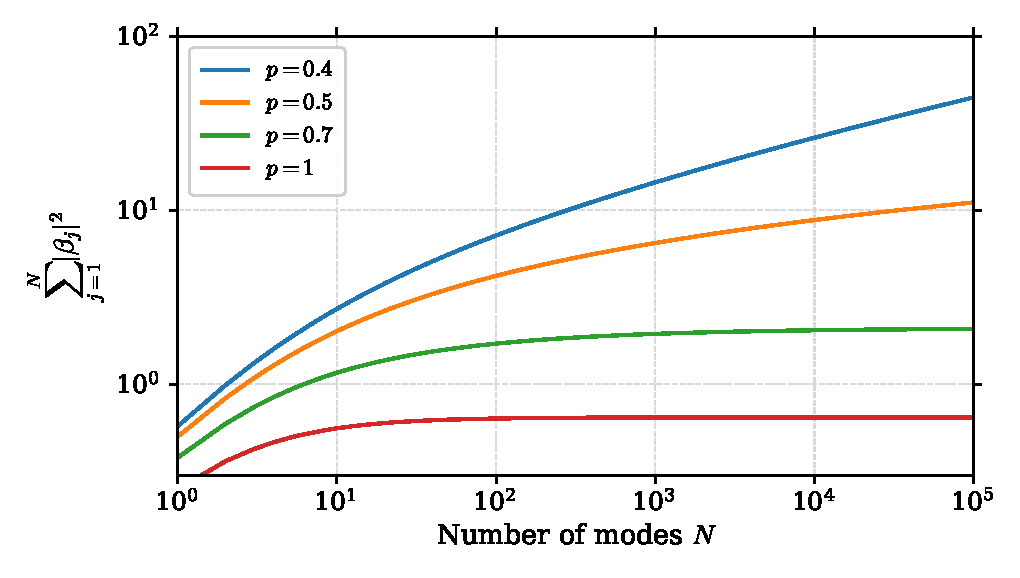
\includegraphics[width=.80\linewidth]{content/FreeElectronQuantumOptics/figures/geometry-highspin/generated/fock_implementability.pdf}
\caption{幂律 $|\beta_j|=(j+1)^{-p}$ 的截断 Hilbert--Schmidt 范数 $\sum_{j\le N}|\beta_j|^2$。图中精确求和展示 $p>1/2$ 的收敛、临界 $p=1/2$ 的对数增长和 $p<1/2$ 的幂律增长；曲线不是连续谱密度的拟合。}
\label{fig:ghs-r7-fock-implementability}
\end{figure}


\subsection{模态偏迹、热态与熵}

对一个模态的中心高斯态，其辛本征值为 $\nu=\sqrt{\det V}\ge\hbar/2$。若它来自双模纯高斯态并将另一个模态迹掉，约化态的平均热占据数可写成 $\bar n=\nu/\hbar-1/2$，其冯诺依曼熵为
\begin{equation}\label{eq:ghs-r6-one-mode-entropy}
S(\rho)=(\bar n+1)\log(\bar n+1)-\bar n\log\bar n.
\end{equation}
当 $\bar n=0$ 时按连续极限取 $0\log0=0$，得到零熵；这与纯态的协方差满足 $\det V=(\hbar/2)^2$ 相符。

这里的 高斯态与后文的双玻色子核状态并非同一种构造。前者由二点协方差及 Wick 性质决定，后者是固定粒子数的 Fock 态，通常不是 高斯态；二者都涉及约化密度矩阵，却不能把两种谱公式混同。一般空间上“粒子数随时间改变”的问题最终应转写成复结构随演化改变的数学问题，而非预设全局球谐量子数。


高斯态可以纯净，也可以在只保留部分模态后变成混态。下面的双模例子无需微分方程或球面坐标，直接显示粒子数分布如何变成熵。设 $r\ge0$，令 $q=\tanh^2r\in[0,1)$，构造两个模式的归一纯态
\begin{equation}\label{eq:ghs-r6-two-mode-squeezed}
|\Psi_r\rangle=\sqrt{1-q}\sum_{n=0}^\infty q^{n/2}|n\rangle_A\otimes|n\rangle_B.
\end{equation}
规范化由等比级数给出：$\langle\Psi_r|\Psi_r\rangle=(1-q)\sum_nq^n=1$。对 $B$ 偏迹时，$\operatorname{Tr}_B(|n\rangle\langle m|)=\delta_{nm}$，因此
\begin{equation}\label{eq:ghs-r6-two-mode-partialtrace}
\rho_A=(1-q)\sum_{n=0}^\infty q^n|n\rangle\langle n|.
\end{equation}
约化态的谱不是假设得到的热谱，而是由 Schmidt 形式严格给出。其平均占据数与纯度分别是
\[
\bar n=(1-q)\sum_{n=0}^\infty nq^n=\frac{q}{1-q}=\sinh^2r,
\quad\operatorname{Tr}\rho_A^2=(1-q)^2\sum_{n=0}^\infty q^{2n}=\frac{1-q}{1+q}.
\]
把 $p_n=(1-q)q^n$ 代入 $-\sum_np_n\log p_n$，又用 $\sum_np_n=1$、$\sum_nnp_n=\bar n$，得到
\[
S(\rho_A)=-\log(1-q)-\bar n\log q
=(\bar n+1)\log(\bar n+1)-\bar n\log\bar n,
\]
恰为 \cref{eq:ghs-r6-one-mode-entropy}。这也说明即使联合态完全纯净，忽略第二个模式仍可留下热形的约化谱；“热形”不要求整个闭合系统经历实际的耗散过程。


\begin{example}[振子的热谱与配分函数]
对单个正频振子，热密度算符定义为 $\rho_\beta=Z^{-1}\ee^{-\beta\widehat H}$，$\beta=(k_{\mathrm B}T)^{-1}$。从 \cref{eq:ghs-r6-oscillator-number} 直接求配分函数
\begin{equation}\label{eq:ghs-r6-oscillator-partition}
Z=\sum_{n=0}^\infty\ee^{-\beta\hbar\omega(n+1/2)}
=\frac{1}{2\sinh(\beta\hbar\omega/2)}.
\end{equation}
进而
\[
\langle N\rangle_\beta=-\frac{\partial}{\partial(\beta\hbar\omega)}
\log(1-\ee^{-\beta\hbar\omega})^{-1}
=\frac{1}{\ee^{\beta\hbar\omega}-1}.
\]
这里直接使用归一几何级数也能得到同一结果，负号来自对 $-\log(1-q)$ 求导时 $q=\ee^{-\beta\hbar\omega}$ 的导数。
\end{example}

为了避免把温度与特殊坐标绑死，可用相关函数的解析性质定义热平衡。在有限维系统中设 $A(t)=\ee^{\ii\widehat Ht/\hbar}A\ee^{-\ii\widehat Ht/\hbar}$。利用迹的循环性得到
\[
\operatorname{Tr}(\rho_\beta A(t)B)
=\operatorname{Tr}(\rho_\beta B A(t+\ii\beta\hbar)),
\]
其含义是关联函数在相应复时间带中满足 Kubo--Martin--Schwinger（KMS）边界条件。核查时把 $t$ 替换成 $t+\ii\beta\hbar$：
\[
A(t+\ii\beta\hbar)=\ee^{-\beta\widehat H}A(t)\ee^{\beta\widehat H},
\]
因此右边的迹等于 $Z^{-1}\operatorname{Tr}(\ee^{-\beta H}B\ee^{-\beta H}A(t)\ee^{\beta H})$，再循环调整即可回到左边。这种以时间自同构和关联函数解析性定义平衡态的方法可以推广到无迹的无穷系统，但解析性与状态存在性必须重新证明。

两模态例子中，若指定 $q=\ee^{-\beta\hbar\omega}$，约化态 \cref{eq:ghs-r6-two-mode-partialtrace} 正好是频率 $\omega$ 的 Gibbs 态。这是在具体 Hilbert 空间中由偏迹产生温度的严格数学对应；它并不说明任何弯曲背景中的观察者都会测到同一温度，因为温度仍依赖所选时间演化生成元。


选择复结构只确定了量子化所需的正频子空间，并不能保证每个所得状态都允许定义局域复合算符。后一个问题取决于二点函数在重合点附近的奇性。


\subsection{Hadamard 态与局域复合算符}

经典双曲方程提供了因果传播与正则对易代数，但不同量子态可能给出极不相同的二点函数。若想在一般曲率背景中讨论局域复合算符、应力张量或高自旋流，首先必须知道二点函数的短距离奇性，并说明可以从中减去哪一部分。量子场的局域性因此不仅是“两个类空分离的算符对易”，还是一种与背景嵌入和局部几何相容的构造原则。


对满足实 Klein--Gordon 方程的量子场，令 $\omega$ 是归一化正态，即 $\omega(A^*A)\ge0$ 且 $\omega(\id)=1$。二点函数是测试函数上的分布
\begin{equation}\label{eq:ghs-r6-two-point-distribution}
W_\omega(f,h)=\omega\bigl(\widehat\phi(f)\widehat\phi(h)\bigr).
\end{equation}
它满足场方程 $W(Pf,h)=W(f,Ph)=0$，正性 $W(\bar f,f)\ge0$，其反对称部分由因果 Green 算子固定。对规范化的实场，若采用 \cref{eq:ghs-r6-causal-green} 的 $E$ 和 \cref{eq:ghs-r6-peierls} 的辛号差，则
\begin{equation}\label{eq:ghs-r6-w-antisymmetric}
W_\omega(f,h)-W_\omega(h,f)=-\ii\int_{\mathcal M}f(Eh)\dd\mu_{g_L}
\end{equation}
这是前述源函数映射与单模正频核共同固定的反对称部分；它不依赖量子态。对称部分才记录不同态的协方差。


任取两个满足同一正则对易关系的量子态，它们的二点函数差只能改变对称部分。

\begin{proposition}[同一场代数上的两点函数差]
设 $W_1,W_2$ 是同一场代数上的两个二点分布，则 $D=W_1-W_2$ 在交换两个变量时是对称的，且满足齐次双变量场方程。
\end{proposition}

\begin{proof}
由于二者的反对称部分都等于同一个因果传播分布，
\[
D(f,h)-D(h,f)=[W_1(f,h)-W_1(h,f)]-[W_2(f,h)-W_2(h,f)]=0.
\]
又因为 $W_i(Pf,h)=W_i(f,Ph)=0$，相减即可得 $D(Pf,h)=D(f,Ph)=0$。但此证明只给出对称性和齐次场方程，并不保证 $D$ 光滑；光滑性需要额外的高频正则性条件。
\end{proof}

对一般分布，函数值可能根本不存在。要判断两个分布能否相乘，仅知道它们在哪些点发散远远不够，还需要知道奇性沿哪些余切方向传播。波前集 $\operatorname{WF}(u)\subset T^*M\setminus\{0\}$ 记录位置与非零协向量组成的奇性对。其局部定义可以通过截断分布的 Fourier 变换表述：如果在 $(x_0,\xi_0)$ 附近存在截断函数 $\chi(x_0)\ne0$，使 $\widehat{\chi u}(\xi)$ 在 $\xi_0$ 周围的锥形邻域内比任意幂次衰减更快，那么该点不属于波前集。

例如分布 $\delta(x)$ 在 $x=0$ 的任意非零 Fourier 方向都不快速衰减，而光滑函数的局部 Fourier 变换在所有锥方向快速衰减。两个奇分布的乘积一般不能任意定义：需要检查它们的波前协向量不会在同一点上相加为零。这一数学限制就是局域量子场重整化中出现接触项与延拓歧义的起点。


不同正频分解给出了不同的真空，但局域可观测量的短距离奇性不能任意改变。控制这一奇性所需的条件由场方程的传播结构和量子态的正频性质共同决定。


在四维全局双曲时空的凸正规邻域内，适当的 Hadamard 二点函数有局部结构
\begin{equation}\label{eq:ghs-r6-hadamard-local}
W_\omega(x,x')=\frac{1}{8\pi^2}
\left[\frac{U(x,x')}{\chi_+(x,x')}
+V(x,x')\log\!\frac{\chi_+(x,x')}{\ell^2}
+H_\omega(x,x')\right].
\end{equation}
$\sigma_L$ 是按 $(+,-,\ldots,-)$ 定义的 Synge 世界函数，令 $\chi=-\sigma_L$，使类空分离时 $\chi>0$。$\chi_+$ 表示 $\chi+\ii0(x^0-x\prime{}^0)$ 的因果边界值；在平直空间它等于 $[r^2-(s-\ii0)^2]/2$，$\ell$ 是任意正长度标度。$U,V$ 由度规、质量与曲率耦合的局部递推决定；$H_\omega$ 是依赖态的光滑部分。该表达在四维使用，其他维度的幂次和对数结构不同，不能照搬系数。



若两种态具有相同的局域短距离奇性结构，相减后便可以考察一个普通的光滑核。

\begin{proposition}[Hadamard 态差的光滑性]
若 $W_1,W_2$ 都是同一个自由场方程的 Hadamard 二点函数，则 $W_1-W_2$ 为光滑双点函数。在固定的局部几何减法方案中，它们的 Wick 平方差因而可以由重合极限直接计算。
\end{proposition}

\begin{proof}
在共同的凸正规邻域内，两者具有相同的 $U/\chi_+$ 和 $V\log(\chi_+/\ell^2)$ 奇异项，这些项由局部几何和场方程决定。相减后只剩 $(H_1-H_2)/(8\pi^2)$，在邻域内光滑。利用双曲方程的局部覆盖和 Hadamard 条件的传播性质，可将该结论延拓到相应全局区域。这里用到了 Hadamard 性质，而不仅是二点函数的对易部分相同。
\end{proof}

因此复合算符 $\phi^2(x)$ 不能简单写成 $\widehat\phi(x)\widehat\phi(x)$，但可以先考虑两点的乘积、减去标准几何奇性，再取 $x'\to x$ 的极限：
\begin{equation}\label{eq:ghs-r6-point-split-wick}
:\!\widehat\phi^2\!:(x)
=\lim_{x'\to x}\left[\widehat\phi(x)\widehat\phi(x')-H_{\mathrm{sing}}(x,x')\id\right],
\end{equation}
其中 $H_{\mathrm{sing}}$ 必须带正确的因果边界值，并仅指奇异的几何部分。在算符值分布意义下，这个极限需通过测试函数理解。允许的局域有限重定义还可以含与量纲匹配的曲率项；故 \cref{eq:ghs-r6-point-split-wick} 并非一个对任何背景都完全无歧义的数值定义。


把 Hadamard 形式抽象地写下以后，最好回到一个可以做完的例子，确认它的系数和短距离尺度。考虑四维 闵可夫斯基时空中 $m=0$ 的标量，令 $s=x^0-x'^0$、$r=|\vb x-\vb x'|$，选择正频真空，则二点函数的 Fourier 积分是
\begin{equation}\label{eq:ghs-r6-flat-vacuum-fourier}
W_0(s,r)=\int_{\RR^3}\frac{\dd^3k}{(2\pi)^3}
\frac{\ee^{-\ii|\vb k|s+\ii\vb k\cdot(\vb x-\vb x')}}{2|\vb k|}.
\end{equation}
积分必须通过 $s\mapsto s-\ii\varepsilon$、$\varepsilon>0$ 的边界值理解。令球极轴沿 $\vb x-\vb x'$，则
\[
\int_{S^2}\ee^{\ii kr\cos\theta}\dd\Omega
=4\pi\frac{\sin kr}{kr}.
\]
因此先积分角度后剩下
\begin{align*}
W_0(s,r)
&=\frac{1}{4\pi^2r}\lim_{\varepsilon\downarrow0}
\int_0^\infty\ee^{-(\varepsilon+\ii s)k}\sin(kr)\dd k\\
&=\frac{1}{4\pi^2r}\lim_{\varepsilon\downarrow0}
\frac{r}{(\varepsilon+\ii s)^2+r^2}.
\end{align*}
使用 $\int_0^\infty\ee^{-ak}\sin(bk)\dd k=b/(a^2+b^2)$（$\operatorname{Re}a>0$），便得到
\begin{equation}\label{eq:ghs-r6-flat-massless-wightman}
W_0(s,r)=\frac{1}{4\pi^2[r^2-(s-\ii0)^2]}.
\end{equation}
它恰好与四维 Hadamard 主项一致：在平直时空 $U=1$、$V=0$，世界函数 $\sigma_L=\tfrac12(s^2-r^2)$，因而 $\chi_+=\tfrac12[r^2-(s-\ii0)^2]$。若遗漏 Fourier 测度中的 $(2\pi)^{-3}$ 或正频模态的 $1/(2|k|)$，该一致性立刻失效。

再看同一场的热态。它比零温真空多出的对称二点函数由 Bose 因子
$n_\beta(k)=(\ee^{\beta\hbar c k}-1)^{-1}$ 决定。在重合点减去真空奇性以后，温度引起的有限增量为
\begin{align*}
\langle:\!\phi^2\!:\rangle_\beta
&=\int_{\RR^3}\frac{\dd^3k}{(2\pi)^3}\frac{n_\beta(k)}{|\vb k|}\\
&=\frac1{2\pi^2}\int_0^\infty\frac{k\dd k}{\ee^{\beta\hbar ck}-1}.
\end{align*}
令 $u=\beta\hbar ck$，再展开 $(\ee^u-1)^{-1}=\sum_{m=1}^\infty\ee^{-mu}$，交换由单调收敛支持的求和与积分，得到
\[
\int_0^\infty\frac{u\dd u}{\ee^u-1}
=\sum_{m=1}^\infty\frac1{m^2}=\frac{\pi^2}{6},
\]
因此
\begin{equation}\label{eq:ghs-r6-thermal-wick-square}
\langle:\!\phi^2\!:\rangle_\beta
=\frac{(k_{\mathrm B}T)^2}{12\hbar^2c^2}.
\end{equation}
这里 $\phi$ 按前文采用的长度维数 $L^{-1}$ 规范化，结果量纲是 $L^{-2}$；若重新赋予场其他常数归一化，数值期望也要相应缩放。零温态与热态的短距离奇性相同，所以二者之差能够在重合点得到有限结果。这是 Hadamard 减法的一个直接、可检验的应用，而非把正规序当作任何曲率背景上天然存在的操作。

\begin{figure}[htbp]
\centering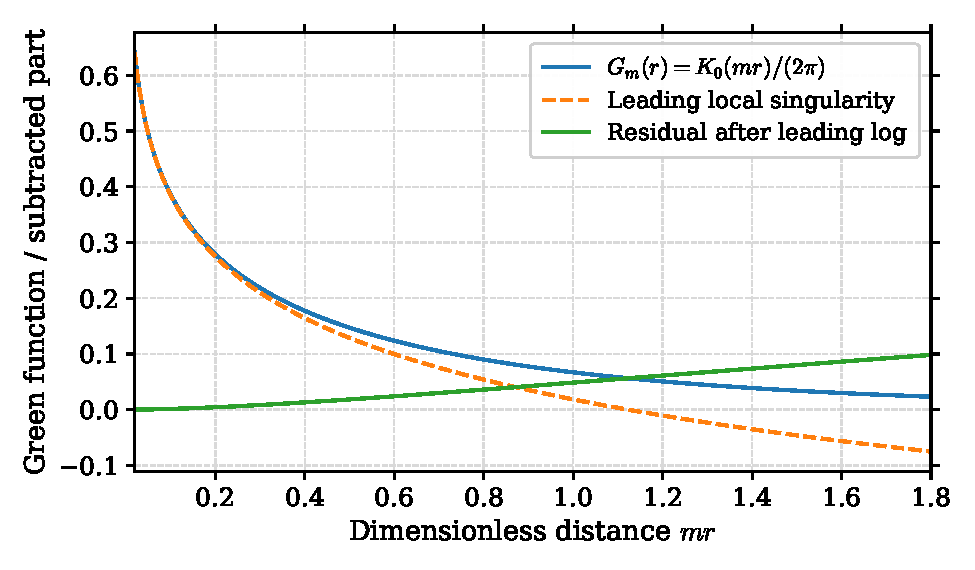
\includegraphics[width=.79\linewidth]{content/FreeElectronQuantumOptics/figures/geometry-highspin/generated/hadamard_bessel_remainder.pdf}
\caption{二维欧氏有质量标量的 Green 核 $G_m(r)=K_0(mr)/(2\pi)$、领先对数奇性 $-[\log(mr/2)+\gamma_E]/(2\pi)$ 及两者之差。剩余项为 $O(r^2\log r)$；只减领先奇性尚不能保证全部阶数光滑。}\label{fig:ghs-hadamard-bessel-remainder}
\end{figure}

\cref{fig:ghs-hadamard-bessel-remainder} 是一个刻意简单的局部模型，不能把二维欧氏系数直接代入四维 Lorentz Hadamard 形式。图中残差趋零，但其二阶导数仍可能含对数奇性。


一般曲率背景不再共享同一个 Poincaré 群，因此不能用“让同一群作用在每个时空上”定义所有场的协变性。更普适的办法是把一个全局双曲时空及其定向、时间定向、度规视为一个对象，将保持这些结构并使因果关系相容的嵌入看作态射。给每个时空 $\mathcal M$ 配置一个局域观测量 $*$-代数 $\mathfrak A(\mathcal M)$，给每个嵌入 $\psi:\mathcal M\hookrightarrow\mathcal N$ 配置单射 $\alpha_\psi:\mathfrak A(\mathcal M)\to\mathfrak A(\mathcal N)$，并要求
\begin{equation}\label{eq:ghs-r6-locally-covariant-functor}
\alpha_{\operatorname{id}}=\operatorname{id},\qquad
\alpha_{\psi_2\circ\psi_1}=\alpha_{\psi_2}\circ\alpha_{\psi_1}.
\end{equation}
这就是局域协变量子场论的一种范畴论表述。\cref{eq:ghs-r6-locally-covariant-functor} 本身只是函子结构；还必须另外提出微因果性、时间片公理和具体动力学条件，才成为充分的物理理论。参见 \cite{ghs-r6-bfv,ghs-r6-fewster-verch}。


在经典层面，作用量对度规的变分定义能动张量。对自由标量场，它包含导数、质量以及 $\xi$ 引入的改进项；曲率背景下，试图用 $\nabla_a\phi\nabla_b\phi$ 的点乘直接定义其量子期望也会碰到 重合点奇性。因此必须先做与 \cref{eq:ghs-r6-point-split-wick} 相容的点分离减法，再对两个变量施加双微分算子。

要求局域协变性、适当缩放律与守恒律后，有限重整化歧义受到严格限制，但一般并不消失。四维理论中，允许的局域曲率张量（在相应质量维数约束下）提供了可能的有限变更。对经典共形耦合的无质量标量，即使经典迹为零，量子迹也可能含曲率不变量构成的异常；因此不能未经分析就把守恒高自旋流在平直背景的性质原封不动搬到任意曲率空间。

综上，一般空间的局域量子场论要求把三种结构分开：几何决定微分算子的主符号与局部奇性，初值问题决定因果传播和对易关系，量子态决定二点函数的光滑部分与实际观测值。只有在三者都明确之后，讨论曲率背景中高自旋复合算符的守恒、混合和反常维数才是一个有定义的问题。

\section{局域短距离结构与尺度异常}

传播算子与正则场代数确定了基本的因果结构，但它们尚未规定复合场在同一点附近应怎样定义。这个困难必须从二点函数的短距离行为入手。


欧氏径向时间是尺度参数，不是实验室的时间。要在一般物理时空中建立量子场，必须先明确因果结构。洛伦兹流形上的基本算子是双曲型，而不是欧氏椭圆型；它的传播子取决于过去或未来的边界条件。两种几何可以通过特定解析延拓联系，但不能把一个任意欧氏流形直接称为量子时空。


一般流形上没有全球尺度对称性，却仍可能存在局域算符乘积展开。它的普适性来自局部微分几何与短距离奇性，而不是全局共形块。这个区别决定了研究重整化场论时哪些结构应该放在最前面：首先要定义局域场的分布核和复合场，再讨论短距离渐近中的算符系数。


量子场 $\widehat\phi(x)$ 是算符值分布，首先对试验函数作用得到 $\widehat\phi(f)$。两点函数 $W(x,y)$ 也是双变量分布；其对角限制 $x=y$ 往往不存在。因此所谓 $\widehat\phi(x)^2$ 不能简单以普通乘法定义。短距离奇性并非技术缺陷，而是量子场局域化的自然结果。

\subsection{基本核、热核与局域算符乘积}

在平直 $d>2$ 欧氏空间，归一化质量为零标量的 Green 核为
\begin{equation}\label{eq:ghs-flat-euclidean-fundamental-solution}
 G_d(x,y)=\frac{\Gamma(d/2-1)}{4\pi^{d/2}}
 |x-y|^{2-d}.
\end{equation}
它满足 $-\Delta_xG_d(x,y)=\delta^{(d)}(x-y)$ 的分布恒等式。常数由小球通量而非猜测确定。


传播子的整体归一化由源点附近的通量条件固定。
令 $G(r)=Cr^{2-d}$。在 $r>0$ 上，径向拉普拉斯给出
$\Delta G=G''+(d-1)G'/r=0$。
对半径 $\varepsilon$ 的球使用 Gauss 定理，
\[
 -\int_{B_\varepsilon}\Delta G\,\dd^dx
 =-\int_{S_\varepsilon}\partial_rG\,\dd\Sigma
 =C(d-2)\Omega_{d-1}.
\]
要等于单位点源，须取 $C=1/[(d-2)\Omega_{d-1}]$。代入 $\Omega_{d-1}=2\pi^{d/2}/\Gamma(d/2)$ 与 Gamma 递推 $\Gamma(d/2)=(d/2-1)\Gamma(d/2-1)$，得到 \cref{eq:ghs-flat-euclidean-fundamental-solution}。这个通量计算同时给出了 $\delta$ 函数归一化的几何来源。


对于无边界紧致黎曼流形上的 Laplace 型算子 $A=-\Delta_g+V$，令 $K(s;x,y)$ 是 $\ee^{-sA}$ 的核。短时、近对角的几何展开形式为
\begin{equation}\label{eq:ghs-heat-kernel-parametrix}
 K(s;x,y)\sim\frac{\ee^{-\sigma(x,y)/(2s)}}{(4\pi s)^{d/2}}
 \Delta_{\rm VV}(x,y)^{1/2}\sum_{k=0}^\infty s^ka_k(x,y).
\end{equation}
$\sigma(x,y)$ 是测地距离平方的一半，$\Delta_{\rm VV}$ 为 Van Vleck 行列式，取 $\Delta_{\rm VV}(x,x)=1$。这个局域展开要求 $x,y$ 位于凸正规邻域；跨过割迹以后不能用单一测地距离函数全局表示 Green 核。

\begin{proposition}[第一项局域热核系数]
\label{prop:ghs-heat-kernel-first}
对标量算子 $A=-\Delta_g+V$，对角系数满足
\begin{equation}\label{eq:ghs-first-heat-coefficient}
 a_0(x,x)=1,\qquad a_1(x,x)=\frac{\mathcal R(x)}6-V(x).
\end{equation}
\end{proposition}
\begin{proof}
将 \cref{eq:ghs-heat-kernel-parametrix} 代入 $(\partial_s+A_x)K=0$，按 $s$ 的幂次比较。最高负次幂给出 Hamilton--Jacobi 方程 $|\nabla_x\sigma|^2=2\sigma$；下一阶的输运方程固定 $a_0(x,y)=1$（Van Vleck 因子已提取在外）。常数阶要求
$\bigl[a_1(x,x)\bigr]=[\Delta_x\Delta_{\rm VV}^{1/2}]-V(x)$。在正规坐标中，$\Delta_{\rm VV}^{1/2}(x,y)=1+\frac1{12}\operatorname{Ric}_{ij}(y)\zeta^i\zeta^j+O(|\zeta|^3)$，取两次平直领先导数得到 $\mathcal R/6$，于是得结果。此证明在局部渐近级数意义成立，不声称级数对固定 $s$ 收敛。
\end{proof}

\begin{proposition}[由正谱热核恢复逆算子]
\begin{equation}\label{eq:ghs-heat-green-laplace}
 A^{-1}=\int_0^\infty\ee^{-sA}\dd s,\qquad A\ge a_0 I>0.
\end{equation}
\end{proposition}
\begin{proof}
在谱值 $\lambda\ge a_0$ 上，$\int_0^\infty\ee^{-s\lambda}\dd s=\lambda^{-1}$。用 $\|\ee^{-sA}\|\le\ee^{-a_0s}$ 控制积分，再按谱定理恢复算子；截断尾部的范数不超过 $\ee^{-a_0S}/a_0$。
\end{proof}
Green 核因此可以通过热核积分恢复。$s\to0$ 的局域行为决定紫外奇性，$s\to\infty$ 的谱下界则决定红外收敛。因此重整化的紫外问题和真空的红外问题在谱语言中有明确不同的来源。


在洛伦兹时空，物理上合理的自由场态通常要求两点函数具有 Hadamard 短距离形式。四维情形在凸正规邻域内可写为
\begin{equation}\label{eq:ghs-hadamard-four-dimensional}
 W(x,y)=\frac1{8\pi^2}\left[
 \frac{U(x,y)}{\chi_+(x,y)}+V(x,y)\log\frac{\chi_+(x,y)}{\ell^2}
 +H(x,y)\right],
\end{equation}
这里 $\chi_+=(-\sigma_L)_+$ 表示与前述正频核相容的因果边界值，$U,V$ 由局部几何及场算子递推确定，$H$ 随量子态改变，$\ell$ 为重整化长度。公式仅针对选定规范与四维标量；任意维的奇偶对数结构必须区别处理。

若两个 Hadamard 态的两点函数之差光滑，可以用某个参考 Hadamard 参数子 $H_{\rm sing}$ 做点分裂正规序：
\[
 :\!\phi^2\!:(x)=\lim_{y\to x}\left[\widehat\phi(x)\widehat\phi(y)-H_{\rm sing}(x,y)\,\id\right].
\]
极限必须在合适的分布/算符值分布意义下，并保留有限局域曲率反项的选择自由。因此复合算符的定义天然包含重整化处方；这部分内容不能由一个形式的 Wick 收缩在所有弯曲空间上直接解决。


在局部协变场论中，若 $x,y\to p$，可考虑渐近形式
\begin{equation}\label{eq:ghs-curved-local-ope}
 \mathcal O_A(x)\mathcal O_B(y)
 \sim\sum_C C_{AB}{}^C(x,y;p;g)\,\mathcal O_C(p),
\end{equation}
系数可以依赖度规、曲率、场参数及点之间的几何输运；当 $\mathcal O_C$ 携带张量指标时还须用平行输运比较不同点的纤维。符号 $\sim$ 指按给定短距离缩放度数逐阶逼近，既不是任意分离点的绝对收敛求和，也不预设存在一个全球标度维数离散谱。

平直共形场论的 OPE 是这套局域结构获得全球共形约束后的特殊情形：其系数由维数、旋转表示与三点函数数据大幅简化，才可以进一步重组为共形块。这也是下一部分为何可以集中研究 $SO(d+1,1)$ 的原因。


\subsection{量子行列式与二维尺度异常}

共形 Laplace 算子的经典 Weyl 协变性，并不保证量子配分函数在 Weyl 变换下不变。特别是在偶数维，重整化后的行列式可以保留局域的尺度异常。在二维，这种异常又与 Virasoro 代数的中心荷和圆柱真空能直接相关，因此不能简单地把前面 $d>2$ 的标量公式代入 $d=2$。


对有限维正矩阵 $A$，高斯积分满足 $\int\dd^Nx\,\ee^{-x^TAx/2}=(2\pi)^{N/2}(\det A)^{-1/2}$。无限维自由场形式上给出 $Z\propto(\det A)^{-1/2}$，但
$\log\det A=\sum_j\log\lambda_j$ 一般发散。若 $A$ 是紧致背景上正定椭圆算子，定义谱 zeta 函数
\begin{equation}\label{eq:ghs-zeta-operator}
 \zeta_A(s)=\sum_{\lambda_j>0}\lambda_j^{-s}
 =\frac1{\Gamma(s)}\int_0^\infty t^{s-1}\operatorname{Tr}(\ee^{-tA})\dd t,
\end{equation}
右侧初始仅在收敛半平面成立，再由热核渐近解析延拓。定义 $\log\det_\zeta A=-\zeta_A'(0)$。零本征值必须从谱和积分中单独剔除，并处理它们的积分测度。


对于二维闭曲面上的正拉普拉斯算子，热核迹为
\[
 \operatorname{Tr}(\ee^{t\Delta_g})
 \sim\frac1{4\pi t}\int_M\left(1+\frac t6\mathcal R_g+O(t^2)\right)\dd\mu_g.
\]
因此正本征值上的 $\zeta_{-\Delta}(0)$ 与局域 $t^0$ 系数有关：
\begin{equation}\label{eq:ghs-zeta-curvature-two-dimensional}
 \zeta_{+,-\Delta}(0)
 =\frac1{24\pi}\int_M\mathcal R_g\dd\mu_g-\dim\ker\Delta_g.
\end{equation}
式中下标 $+$ 表示排除零模后的正本征值谱；该等式来自短时热核常数项与零模修正。

若将度规作常数 Weyl 变换 $g\mapsto\ee^{2\sigma}g$，正特征值按 $\lambda\mapsto\ee^{-2\sigma}\lambda$ 缩放，所以
\[
 \zeta_{\widehat A}(s)=\ee^{2\sigma s}\zeta_A(s),\qquad
 \log\det_\zeta\widehat A
 =\log\det_\zeta A-2\sigma\zeta_A(0).
\]
这说明经典算子的共形协变与量子配分函数的尺度不变性是两个不同命题；一个有限的局域热核系数就足以留下异常。对局域非均匀 Weyl 变换，还须分析位置依赖的热核系数与所选反项。


\begin{proposition}[二维圆柱的异常真空能]
在二维共形理论中，中心荷记为 $c_{\rm CFT},\overline c_{\rm CFT}$。用复平面坐标 $z$ 和无量纲圆柱坐标 $w=\log z$，全纯应力张量变换为
\begin{equation}\label{eq:ghs-stress-schwarzian}
 T_{ww}(w)=\left(\frac{\dd z}{\dd w}\right)^2T_{zz}(z)
 +\frac{c_{\rm CFT}}{12}\{z,w\},\qquad
 \{z,w\}=\frac{z'''}{z'}-\frac32\left(\frac{z''}{z'}\right)^2.
\end{equation}
圆柱空间半径为 $R$ 时，绝对能量为
\begin{equation}\label{eq:ghs-virasoro-cylinder-hamiltonian}
 H_{\rm cyl}=\frac{\hbar c}{R}\left(L_0+\overline L_0-
 \frac{c_{\rm CFT}+\overline c_{\rm CFT}}{24}\right).
\end{equation}
\end{proposition}
\begin{proof}
应力张量的异常变换式以二维 Ward 恒等式和中心扩张为输入。对 $z=\ee^w$，所有阶导数相同，故 $\{z,w\}=1-3/2=-1/2$。平面真空 $\langle T_{zz}\rangle=0$ 给出 $\langle T_{ww}\rangle=-c_{\rm CFT}/24$，反全纯部分给出 $-\overline c_{\rm CFT}/24$。两部分的零模之和是无量纲时间平移生成元，乘以 $\hbar c/R$ 恢复物理 哈密顿量。
\end{proof}
若左右中心荷相等，真空能为 $-\hbar c\,c_{\rm CFT}/(12R)$。尺度生成元对应圆柱相对真空的激发能隙，绝对真空能还包含异常位移。

当 $d=2$ 时，共形标量权重 $\delta=(d-2)/2=0$，圆周 Laplace 算子存在常数零模。质量为零的非紧致自由标量不仅缺少有界的 $A^{-1/2}$，其两点函数也呈对数行为而非 $r^{2-d}$。所以二维共形场论通常更自然地研究导数场、顶点算符及恰当处理零模后的扇区；这些结构不能通过把高维的 $\ell+\delta$ 频率公式机械取极限得到。

对于偶数高维，Weyl 异常由相应维数的热核系数组织；对于奇数维闭合光滑背景，通常没有同类局域体内 Weyl 异常，但边界、缺陷、整体拓扑和重整化条件仍可能引入其他异常。这些限定使前面的任意维几何论证不会掩盖量子层面的真实差异。

欧氏的热半群不能代替真实时间的演化。洛伦兹场方程首先决定经典的 Cauchy 演化及守恒辛形式；选择何种量子态则是随后才出现的另一个问题。



边界核与因果场代数已经区分了几何数据、正频选择和局域减法。下一章取满足反射正性与共形对称的平直真空扇区，在球面上构造局域算符产生的态；其中的角动量与单体约化谱将由这里的谱量子化和双玻色核计算共同确定。
